\documentclass[11pt,a4paper]{article}

% ===================== ENCODING & LANGUAGE =====================
\usepackage[T1]{fontenc}
\usepackage[utf8]{inputenc}
\usepackage[italian]{babel}

% ===================== FONTS (editorial) =====================
\usepackage{mathpazo}                 % Palatino body + math
\usepackage[scaled=0.90]{helvet}      % Helvetica-like sans for headings
\usepackage{courier}
\usepackage[final]{microtype}

% ===================== GEOMETRY =====================
\usepackage[a4paper,top=2.6cm,bottom=2.6cm,left=2.5cm,right=2.5cm,headheight=15pt]{geometry}

% ===================== GRAPHICS / COLOR =====================
\usepackage[table]{xcolor}
\usepackage{tikz}
\usetikzlibrary{positioning,arrows.meta,shapes.geometric,calc,backgrounds,fit}
\usepackage{pgfplots}
\pgfplotsset{compat=1.18}
\usepgfplotslibrary{groupplots}
\usepackage{pgf-pie}

% ===================== TABLES =====================
\usepackage{booktabs}
\usepackage{array}
\usepackage{tabularx}
\usepackage{multirow}
\usepackage{makecell}
\renewcommand{\arraystretch}{1.25}

% ===================== LISTS / MISC =====================
\usepackage{enumitem}
\setlist{itemsep=2pt,topsep=3pt,parsep=0pt}
\usepackage{tcolorbox}
\tcbuselibrary{skins,breakable}
\usepackage{fancyhdr}
\usepackage{titlesec}
\usepackage{caption}
\usepackage{amsmath,amssymb}
\usepackage{lastpage}

% ===================== PALETTE =====================
\definecolor{primary}{HTML}{17435A}    % deep petrol
\definecolor{secondary}{HTML}{2C7A7B}  % teal
\definecolor{accent}{HTML}{B0772A}     % amber/ochre
\definecolor{passgreen}{HTML}{2F7D55}
\definecolor{gapred}{HTML}{9B2C2C}
\definecolor{partial}{HTML}{B0772A}
\definecolor{inkgray}{HTML}{3A3F43}
\definecolor{softbg}{HTML}{F3F6F7}
\definecolor{rulec}{HTML}{C9D6DA}
\definecolor{codebg}{HTML}{F5F2EC}
\definecolor{primaryblue}{HTML}{17435A} % alias per la tabella benchmark
\definecolor{roweven}{HTML}{F3F6F7}     % alias per la tabella benchmark

\color{inkgray}

% ===================== HYPERREF =====================
\usepackage[colorlinks=true,linkcolor=primary,citecolor=secondary,urlcolor=secondary]{hyperref}

% ===================== SECTION STYLING =====================
\titleformat{\section}
  {\sffamily\Large\bfseries\color{primary}}
  {\thesection}{0.7em}{}[\vspace{2pt}{\color{rulec}\titlerule[1.2pt]}]
\titleformat{\subsection}
  {\sffamily\large\bfseries\color{secondary}}
  {\thesubsection}{0.6em}{}
\titleformat{\subsubsection}
  {\sffamily\normalsize\bfseries\color{inkgray}}
  {\thesubsubsection}{0.5em}{}
\titlespacing*{\section}{0pt}{16pt}{8pt}
\titlespacing*{\subsection}{0pt}{12pt}{4pt}

% Part headers
\titleformat{\part}[display]
  {\sffamily\bfseries\color{primary}}
  {\filright\Large PARTE \thepart}{6pt}{\Huge}
\titlespacing*{\part}{0pt}{0pt}{10pt}

% ===================== HEADER / FOOTER =====================
\pagestyle{fancy}
\fancyhf{}
\renewcommand{\headrulewidth}{0.4pt}
\renewcommand{\footrulewidth}{0pt}
\fancyhead[L]{\footnotesize\sffamily\color{primary}GraphRAG per Molecular Tumor Board}
\fancyhead[R]{\footnotesize\sffamily\color{inkgray}\leftmark}
\fancyfoot[C]{\footnotesize\sffamily\color{inkgray}\thepage\ / \pageref{LastPage}}
\renewcommand{\sectionmark}[1]{\markboth{#1}{}}

% ===================== TCOLORBOX STYLES =====================
\newtcolorbox{insightbox}[1][]{
  enhanced, breakable, colback=softbg, colframe=secondary,
  boxrule=0pt, leftrule=3pt, arc=2pt, left=10pt, right=10pt, top=7pt, bottom=7pt,
  fonttitle=\sffamily\bfseries\color{secondary},
  coltitle=secondary, title={#1}}

\newtcolorbox{defbox}[1][]{
  enhanced, breakable, colback=white, colframe=primary,
  boxrule=0.8pt, arc=2pt, left=10pt, right=10pt, top=7pt, bottom=7pt,
  fonttitle=\sffamily\bfseries\color{white}, coltitle=white,
  colbacktitle=primary, title={#1}, attach boxed title to top left={xshift=8pt,yshift=-2pt},
  boxed title style={boxrule=0pt,arc=1pt}}

\newtcolorbox{warnbox}[1][]{
  enhanced, breakable, colback=gapred!4, colframe=gapred,
  boxrule=0pt, leftrule=3pt, arc=2pt, left=10pt, right=10pt, top=7pt, bottom=7pt,
  fonttitle=\sffamily\bfseries\color{gapred}, coltitle=gapred, title={#1}}

\newtcolorbox{tesibox}[1][Testo per la tesi]{
  enhanced, breakable, colback=accent!6, colframe=accent,
  boxrule=0pt, leftrule=3pt, arc=2pt, left=10pt, right=10pt, top=7pt, bottom=7pt,
  fonttitle=\sffamily\bfseries\color{accent}, coltitle=accent, title={#1}}

\newtcolorbox{quotebox}{
  enhanced, breakable, colback=softbg, colframe=rulec,
  boxrule=0pt, leftrule=2.5pt, arc=1pt, left=10pt, right=10pt, top=5pt, bottom=5pt,
  fontupper=\itshape}

% Code-ish box for Cypher/JSON
\newtcolorbox{codebox}[1][]{
  enhanced, breakable, colback=codebg, colframe=accent!55,
  boxrule=0.6pt, arc=1.5pt, left=8pt, right=8pt, top=5pt, bottom=5pt,
  fontupper=\small\ttfamily, title={#1}, fonttitle=\sffamily\bfseries\footnotesize\color{accent},
  coltitle=accent}

% ===================== HELPER MACROS =====================
\newcommand{\pa}{\,\textcolor{secondary}{\textrightarrow}\,}
\newcommand{\code}[1]{\texttt{\small #1}}
\newcommand{\bench}[1]{\texttt{\small #1}}
\newcommand{\fail}[1]{\textcolor{gapred}{\bfseries #1}}
\newcommand{\pass}[1]{\textcolor{passgreen}{\bfseries #1}}
\newcommand{\passstatus}{\textbf{\color{passgreen}PASS}}
\newcommand{\parz}{\textbf{\color{partial}PARZIALE}}
\newcommand{\gap}{\textbf{\color{gapred}GAP}}

% ===================== TITLE PAGE DATA =====================
\begin{document}
\sloppy

% ========================================================
% TITLE PAGE
% ========================================================
\begin{titlepage}
\thispagestyle{empty}
\centering
\vspace*{1.2cm}

{\color{rulec}\rule{\textwidth}{1.2pt}}\\[6pt]
{\sffamily\small\color{secondary}\bfseries TESI MAGISTRALE \,\textbullet\, INGEGNERIA INFORMATICA}\\[2pt]
{\sffamily\footnotesize\color{inkgray}Universit\`a della Calabria}\\[10pt]
{\color{rulec}\rule{\textwidth}{0.6pt}}\\[28pt]

{\sffamily\bfseries\color{primary}\fontsize{30}{34}\selectfont Sistema GraphRAG Agentico\\[6pt] per Molecular Tumor Board}\\[16pt]

{\sffamily\large\color{secondary} Report del lavoro svolto}\\[4pt]
{\sffamily\normalsize\color{inkgray} Dalla Knowledge Base alla campagna sperimentale su RQ1}\\[6pt]
{\sffamily\footnotesize\color{inkgray} Periodo: 29 maggio --- 8 giugno 2026}\\[34pt]

% Stat banner
\begin{tcolorbox}[enhanced,width=0.92\textwidth,colback=softbg,colframe=primary,
  boxrule=0.8pt,arc=3pt,left=14pt,right=14pt,top=12pt,bottom=12pt]
\centering\sffamily
{\color{primary}\bfseries Stato del progetto}\\[8pt]
\begin{tabularx}{\textwidth}{>{\centering\arraybackslash}X >{\centering\arraybackslash}X >{\centering\arraybackslash}X}
{\Large\bfseries\color{secondary}9 / 11} & {\Large\bfseries\color{secondary}30 / 30} & {\Large\bfseries\color{secondary}100\%}\\[2pt]
{\footnotesize tipi di nodo / relazione} & {\footnotesize casi benchmark coperti} & {\footnotesize integrit\`a referenziale}\\[10pt]
{\Large\bfseries\color{accent}3.96 / 5} & {\Large\bfseries\color{accent}100\%} & {\Large\bfseries\color{accent}0\%}\\[2pt]
{\footnotesize score medio (rubrica v2)} & {\footnotesize Evidence Grounding (+ Enricher)} & {\footnotesize allucinazione PMID zero-shot}\\
\end{tabularx}
\end{tcolorbox}

\vfill
{\color{rulec}\rule{\textwidth}{0.6pt}}\\[6pt]
{\sffamily\footnotesize\color{inkgray} Documento di sintesi tecnica --- versione per la discussione con il relatore}\\[2pt]
{\sffamily\footnotesize\color{inkgray} Pipeline FastAPI \,\textbullet\, LangGraph \,\textbullet\, Neo4j \,\textbullet\, React}
\end{titlepage}

% ========================================================
% EXECUTIVE SUMMARY
% ========================================================
\section*{Sommario esecutivo}
\addcontentsline{toc}{section}{Sommario esecutivo}
\markboth{Sommario esecutivo}{}

Questo report consolida il lavoro tecnico e metodologico svolto nell'arco di due settimane sul sistema oggetto della tesi: una \textbf{pipeline agentica GraphRAG} per il supporto decisionale al Molecular Tumor Board (MTB) in oncologia di precisione. Il punto di partenza era un Knowledge Graph (KG) oncologico gi\`a costruito e caricato in Neo4j; il punto di arrivo \`e una pipeline multi-agente completa, end-to-end, valutata sistematicamente su un benchmark clinico di 30 casi reali.

Il percorso si articola in cinque blocchi logici, che corrispondono alle parti di questo documento: (i) il \emph{consolidamento infrastrutturale} del KG e il suo audit quantitativo; (ii) la \emph{costruzione del benchmark} clinico e la sua validazione sul grafo; (iii) l'\emph{architettura multi-sorgente} che integra CIViC e OncoKB; (iv) il \emph{disegno della pipeline} agentica e il suo posizionamento rispetto allo stato dell'arte; (v) la \emph{metodologia di valutazione} e i risultati sperimentali che rispondono alle domande di ricerca.

\begin{insightbox}[I tre risultati che blindano la tesi]
\begin{enumerate}[leftmargin=1.4em]
\item \textbf{Verificabilit\`a citazionale.} Il modello zero-shot allucina il 100\% delle citazioni (115/115 PMID non pertinenti o inesistenti); il GraphRAG con Enricher raggiunge il 100\% di Evidence Grounding, garantendo la tracciabilit\`a totale delle fonti.
\item \textbf{Sicurezza clinica multi-sorgente.} Il routing CIViC\,+\,OncoKB corregge evidenze fuorvianti (caso \bench{013}, ALK G1202R) che un agente mono-sorgente avrebbe scartato, con un impatto di sicurezza clinica diretto.
\item \textbf{Knowledge fall-back.} L'arricchimento live via OncoKB risolve i gap strutturali del database locale (+3.35 di score sul caso ALK G1202R), confermando il valore dell'architettura ibrida.
\end{enumerate}
\end{insightbox}

\vspace{4pt}
\noindent\textit{Nota.} Tutte le cifre, i conteggi e i risultati riportati provengono dai log di sessione del progetto. Le citazioni testuali dai paper di riferimento sono riportate tra virgolette con autore/anno; il resto \`e parafrasi o analisi originale.

\clearpage
\tableofcontents
\clearpage

% ========================================================
% PART I
% ========================================================
\part{Contesto e cronologia}

\section{Introduzione e contesto}

\subsection{Il problema clinico}
In oncologia di precisione, il referto di un test genomico di nuova generazione (NGS) contiene decine di alterazioni molecolari, ciascuna potenzialmente associata a una terapia approvata, a un farmaco off-label, a un trial clinico aperto o a un meccanismo di resistenza noto. La valutazione collegiale di queste informazioni avviene nel \textbf{Molecular Tumor Board (MTB)}, una riunione multidisciplinare di oncologi, biologi molecolari, patologi e bioinformatici.

Il problema operativo \`e che preparare un singolo caso per il MTB richiede ore di lavoro manuale: consultare OncoKB e CIViC, cercare trial su ClinicalTrials.gov, leggere la letteratura su PubMed e assegnare i livelli di evidenza secondo classificazioni come ESCAT. I database curati sono affidabili ma richiedono interrogazioni manuali nodo per nodo; i modelli linguistici producono sintesi fluide ma possono allucinare, mescolano evidenze di livelli diversi e non citano in modo verificabile. Un sistema GraphRAG ben progettato pu\`o unire i vantaggi di entrambi.

\subsection{La soluzione proposta}
Il sistema \`e una pipeline agentica multi-stadio che riceve in input il profilo molecolare di un paziente e produce in output una raccomandazione terapeutica strutturata, con livelli di evidenza espliciti e citazioni verificabili. La componente centrale \`e un Knowledge Graph costruito in Neo4j: gli agenti specializzati lo interrogano con query Cypher invece di generare risposte dalla memoria parametrica di un LLM.

\begin{quotebox}
Il KG \`e come una biblioteca specializzata ben indicizzata. Gli agenti sono bibliotecari esperti che sanno esattamente dove cercare. L'LLM \`e il redattore che trasforma i risultati della ricerca in un report leggibile: senza la biblioteca, il redattore \`e costretto a inventare.
\end{quotebox}

\subsection{Domande di ricerca}
Il lavoro \`e guidato da quattro domande di ricerca:

\begin{defbox}[Domande di ricerca]
\begin{description}[leftmargin=3.2em,style=nextline,font=\bfseries\color{primary}]
\item[RQ1] Il sistema agentico \`e pi\`u accurato e \emph{verificabile} di un LLM zero-shot nel produrre raccomandazioni terapeutiche su casi MTB pubblicati?
\item[RQ2] Il sistema assegna i livelli ESCAT in modo riproducibile e con citazioni verificabili (\emph{faithfulness})?
\item[RQ3] Quanta parte della preparazione del MTB pu\`o essere automatizzata?
\item[RQ4] Un router agentico che attiva dinamicamente solo gli agenti rilevanti migliora precisione e latenza rispetto a una pipeline sequenziale fissa?
\end{description}
\end{defbox}

\subsection{Cronologia sintetica del lavoro}
Il lavoro delle due settimane si dispiega lungo dieci sessioni, riassunte nella linea temporale seguente.

\begin{center}
\begin{tikzpicture}[
  every node/.style={font=\sffamily},
  ms/.style={circle,fill=secondary,inner sep=2.6pt},
  dt/.style={anchor=east,font=\sffamily\bfseries\small\color{primary}},
  tx/.style={anchor=west,font=\sffamily\small\color{inkgray},text width=10.8cm}]
\def\sy{-1.18}
\draw[line width=1.4pt,rulec] (0,0.5) -- (0,11.5*\sy+0.5);
\foreach \i/\d/\t in {
  0/29 mag/{KB oncologica completata e caricata in Neo4j: \textbf{41.426 nodi}, \textbf{51.616 archi}, 7 tipi di nodo, 9 relazioni, integrit\`a referenziale al 100\%.},
  1/30 mag/{Data exploration quantitativa della KB (notebook Jupyter): struttura, copertura clinica, qualit\`a per il benchmark, gap, analisi per il Trial Matcher.},
  2/31 mag/{Primo benchmark di 10 casi MTB (tutti ESCAT Tier I-A) e aggiunta dei nodi \emph{Disease} e \emph{Publication}: tutti i 10 PMID benchmark entrano nel grafo.},
  3/1 giu/{Estensione del benchmark da 10 a 30 casi su 5 categorie cliniche; validazione Cypher (20 PASS, 5 PARZIALI, 5 GAP) e audit scientifico del notebook.},
  4/2 giu/{Note metodologiche sulla valutazione (rubrica + LLM-as-judge); integrazione \textbf{OncoKB} che risolve gli ultimi gap: copertura \textbf{30/30}.},
  5/4 giu/{Incontro con il relatore: riflessioni sui quattro paper di riferimento e gerarchia delle metriche di valutazione.},
  6/5 giu/{Progettazione della pipeline agentica (v1\,$\to$\,v2\,$\to$\,v3), studio delle API OncoKB e formalizzazione dello schema di input clinico.},
  7/6 giu/{Verifica sistematica delle query Cypher per tutti i 6 tipi di \code{alteration\_type}: KB pronta al 100\% per l'integrazione con l'LLM.},
  8/7 giu/{Sistema end-to-end attivo (FastAPI + LangGraph + React); ricalibrazione del judge a 4 criteri e ricalcolo del benchmark; confronto RQ1.},
  9/8 giu/{Risultati finali: allucinazione PMID zero-shot al 100\%, mitigazione del retrieval pollution, validazione dell'Enricher. RQ1 blindato.}}{
    \node[ms] (m\i) at (0,\i*\sy) {};
    \node[dt] at (-0.35,\i*\sy) {\d};
    \node[tx] at (0.35,\i*\sy) {\t};
}
\end{tikzpicture}
\end{center}

% ========================================================
% PART II
% ========================================================
\part{Infrastruttura: Knowledge Graph e audit}

\section{Costruzione del Knowledge Graph}

\subsection{Sorgenti dati}
Il grafo integra sei database pubblici, tutti open access e ampiamente usati nella ricerca clinica internazionale.

\begin{description}[leftmargin=1.4em,font=\bfseries\color{secondary}]
\item[CIViC] Clinical Interpretation of Variants in Cancer: evidenze cliniche sulle varianti genomiche, con livello di evidenza e PMID citabile. Scaricati quattro file TSV (evidenze accettate, varianti, profili molecolari, feature).
\item[DGIdb] Drug-Gene Interaction Database: interazioni farmaco-gene aggregate da una trentina di sorgenti.
\item[OncoKB Cancer Gene List] Lista curata da Memorial Sloan Kettering dei geni oncologici clinicamente rilevanti.
\item[FDA Oncology Therapies] Terapie oncologiche approvate FDA con classificazione precision oncology e biomarker richiesto.
\item[FDA Companion Diagnostic Devices] Dispositivi diagnostici companion (CDx) approvati FDA.
\item[ClinicalTrials.gov] Registro pubblico (API v2): trial oncologici attivi/in reclutamento per 38 geni principali. \textbf{5.570} trial unici dopo deduplicazione su NCT ID (da 9.389 record raw).
\end{description}

In totale sono stati ispezionati 11 file iniziali (TSV ed Excel) per oltre 400.000 righe di dati grezzi, pi\`u il dump di ClinicalTrials.gov.

\subsection{Pulizia dei dati e anomalie risolte}
L'ispezione preliminare ha evidenziato sei anomalie che avrebbero compromesso la qualit\`a del grafo. Sono riepilogate qui sotto.

\begin{center}
\small
\begin{tabularx}{\textwidth}{@{}>{\bfseries\color{primary}}l X@{}}
\toprule
Anomalia & Diagnosi e correzione \\
\midrule
Colonne shiftate CIViC & Pandas leggeva la prima colonna come indice di riga, spostando tutte le altre di una posizione (gli ID contenevano URL e viceversa). Risolto con \code{index\_col=False}. \\
Farmaci duplicati DGIdb & 81.572 righe per soli 24.501 farmaci unici (un alias per sorgente). Deduplicato su \code{concept\_id}. \\
Scope oncologico DGIdb & 98.239 interazioni includevano farmaci cardiologici/psichiatrici. Filtrate a 25.589 mantenendo \code{anti\_neoplastic=True} o gene in cancer gene list. \\
Celle multi-valore CIViC & Colonne \code{therapies}, \code{nct\_ids}, \code{aliases} esplose con \code{df.explode()}: ogni elemento diventa un arco. \\
Null strutturali FDA xlsx & 52\% di null su \code{biomarker}: non un errore, ma assenza fisiologica per i chemioterapici. Caricato il subset precision oncology. \\
Matching nomi farmaci & CIViC usa nomi misti, DGIdb uppercase. Normalizzato (strip\,+\,uppercase); 405 occorrenze non risolvibili salvate in log per revisione manuale. \\
\bottomrule
\end{tabularx}
\end{center}

\subsection{Lo schema del grafo}
Lo schema definitivo, dopo l'aggiunta dei nodi \emph{Disease} e \emph{Publication} (31 maggio), conta \textbf{9 tipi di nodo} e \textbf{11 tipi di relazione}.

\begin{center}
\small
\begin{minipage}[t]{0.49\textwidth}
\centering\sffamily\bfseries\color{primary}\small Tipi di nodo\\[3pt]
\begin{tabular}{@{}lr@{}}
\toprule
Nodo & Quantit\`a \\
\midrule
Drug & 24.501 \\
ClinicalTrial & 5.570 \\
Evidence & 4.843 \\
Publication & 2.222 \\
Variant & 1.973 \\
MolecularProfile & 1.937 \\
Gene & 1.436 \\
Disease & 334 \\
CompanionDiagnostic & 166 \\
\bottomrule
\end{tabular}
\end{minipage}\hfill
\begin{minipage}[t]{0.49\textwidth}
\centering\sffamily\bfseries\color{primary}\small Tipi di relazione\\[3pt]
\begin{tabular}{@{}lr@{}}
\toprule
Relazione & Archi \\
\midrule
INTERACTS\_WITH & 25.589 \\
TESTS\_DRUG & 8.018 \\
ASSOCIATED\_GENE & 5.501 \\
CITED\_IN & 4.840 \\
HAS\_DISEASE & 4.684 \\
HAS\_EVIDENCE & 4.843 \\
TARGETS\_DRUG & 3.347 \\
IN\_MOLECULAR\_PROFILE & 2.279 \\
HAS\_VARIANT & 1.725 \\
DIAGNOSES\_GENE / HAS\_COMP.\_DIAG. & 163 / 150 \\
\bottomrule
\end{tabular}
\end{minipage}
\end{center}

\vspace{4pt}
Il nodo \textbf{Drug} \`e il pi\`u connesso del grafo: riceve relazioni da cinque direzioni diverse (Evidence, Gene via CIViC, Gene via DGIdb, CompanionDiagnostic, ClinicalTrial). \`E il punto centrale attorno a cui ruota tutta la conoscenza terapeutica.

\subsection{La topologia clinica del Knowledge Graph}
Come visibile nello schema (Figura \ref{fig:kbschema}), il modello dati non si limita al tracciamento diretto tra mutazione e terapia, ma implementa una topologia complessa a multi-hop che riflette le reali dipendenze dell'oncologia di precisione.

\begin{itemize}
\item \textbf{Il percorso biologico-clinico (6-Hop):} Il cammino principale (asse centrale) parte dal \code{Gene}, transita fisiologicamente per la \code{Variant} e il suo \code{MolecularProfile}, agganciandosi infine alla \code{Clinical Evidence}. \`E solo a questo livello --- quello dell'evidenza clinica --- che il grafo si dirama simultaneamente verso il farmaco (\code{TARGETS\_DRUG}), la patologia bersaglio (\code{HAS\_DISEASE}) e la fonte scientifica di supporto (\code{CITED\_IN}). Questa catena impedisce le associazioni fuori contesto.
\item \textbf{Interazioni Farmacodinamiche Dirette:} La relazione \code{INTERACTS\_WITH} collega direttamente \code{Gene} e \code{Drug}, catturando i dati crudi di interazione molecolare di DGIdb (1-Hop).
\item \textbf{Trial Matcher e Diagnostica:} L'ecosistema integra i \code{Clinical Trial}, mappati contemporaneamente ai geni (\code{ASSOCIATED\_GENE}) e ai farmaci sperimentali (\code{TESTS\_DRUG}); in modo speculare, i \code{Companion Diagnostic} correlano il farmaco al test genomico specifico (\code{DIAGNOSES\_GENE}).
\end{itemize}

\begin{figure}[htbp]
\centering
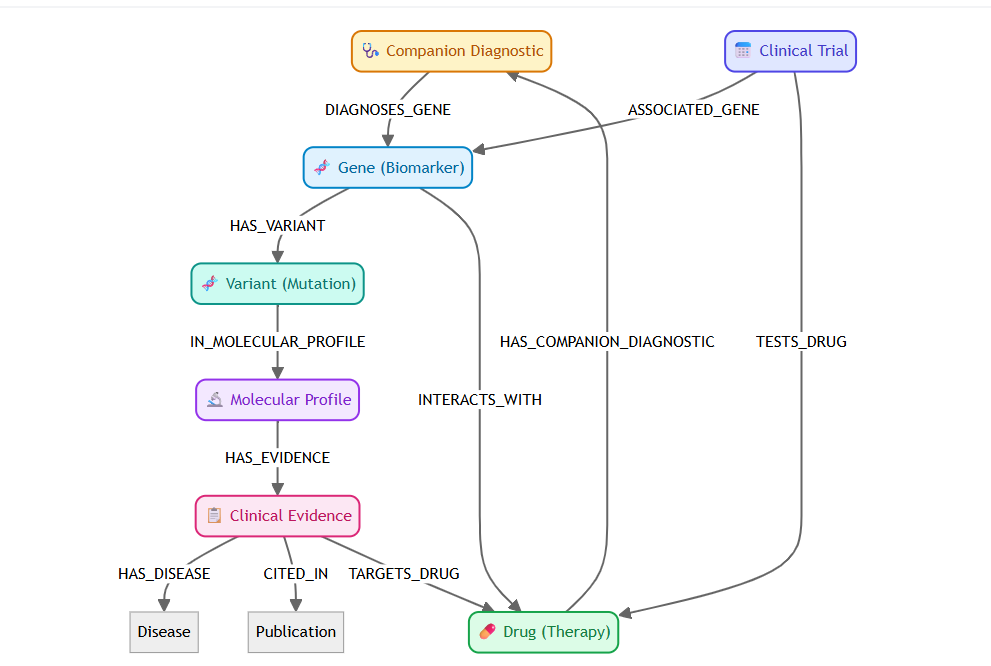
\includegraphics[width=0.90\textwidth]{kb_schema.png}
\caption{Schema topologico del Knowledge Graph oncologico in uso}
\label{fig:kbschema}
\end{figure}

\subsection{Integrit\`a referenziale e caricamento in Neo4j}
Dopo l'ingestion in Neo4j Desktop 5.x (istanza locale \code{GraphRAGTesi}) sono stati creati i constraint di unicit\`a e gli indici sugli attributi di lookup frequente (\code{hugo\_symbol}, \code{drug\_name}). Lo script di verifica ha accertato il \textbf{100\% di allineamento referenziale}: ogni arco punta a nodi che esistono realmente, nessun riferimento rotto, nessun ID orfano --- l'equivalente di un database relazionale senza foreign key violations.

\subsection{Validazione con query reali}
Il grafo \`e stato validato sul caso clinico pi\`u rappresentativo della tesi (NSCLC, EGFR L858R). La query del Variant Interpreter restituisce in 657\,ms i farmaci con evidenza di livello A, ciascuno ancorato al PMID della pubblicazione di supporto.

\begin{codebox}[Cypher --- Variant Interpreter + Target Identifier (EGFR L858R)]
MATCH (g:Gene \{hugo\_symbol:"EGFR"\})\\
\ -[:HAS\_VARIANT]->(v:Variant \{variant\_name:"L858R"\})\\
\ -[:IN\_MOLECULAR\_PROFILE]->(mp:MolecularProfile)\\
\ -[:HAS\_EVIDENCE]->(e:Evidence)\\
\ -[:TARGETS\_DRUG]->(d:Drug)\\
WHERE e.evidence\_level = "A" AND e.evidence\_type = "Predictive"\\
\ \ AND e.significance CONTAINS "Sensitivity"\\
RETURN g.hugo\_symbol, v.variant\_name, mp.name, e.citation\_id, d.drug\_name;
\end{codebox}

\noindent Risultato: \emph{Afatinib, Dacomitinib, Osimertinib, Erlotinib, Gefitinib, Ramucirumab}, ciascuno con PMID verificabile. Sono stati validati anche i casi BRCA1/BRCA2 (PARP inhibitor), BRAF V600E (melanoma vs CRC con significance opposta), BCR::ABL1 (CML) e i companion diagnostic.

\section{Esplorazione e audit della Knowledge Base}

\subsection{Data exploration quantitativa}
\`E stato prodotto un notebook Jupyter che opera direttamente sui CSV puliti, articolato in cinque macro-sezioni pi\`u due analisi aggiuntive (matrice gene-tumore e benchmark Gold per tipo tumorale). I risultati pi\`u rilevanti:

\begin{itemize}
\item \textbf{Distribuzione nodi:} Drug domina con il 60.6\% dei nodi, seguito da ClinicalTrial (13.8\%) ed Evidence (12\%).
\item \textbf{Top geni per varianti:} VHL (313), EGFR (131), TP53 (113), PIK3CA (85), ABL1 (68).
\item \textbf{Top profili per evidenze CIViC:} BRAF V600E (95), ERBB2 Amplification (65), KRAS Mutation (45), PIK3CA Mutation (40), EGFR L858R (37).
\item \textbf{Tipo di evidenza:} Predictive domina con il 58.7\% (2.843 evidenze) --- il tipo direttamente utile alle raccomandazioni del MTB.
\item \textbf{Coerenza biologica:} la matrice gene-tumore conferma i pattern attesi (ABL1 in CML, EGFR in NSCLC, KIT in GIST, FLT3 in AML, PIK3CA trasversale), validazione indiretta della qualit\`a del grafo.
\end{itemize}

\subsection{Riqualificazione scientifica del notebook}
A seguito delle critiche metodologiche del relatore, il notebook \`e stato sottoposto a un audit completo. Erano emerse vulnerabilit\`a che avrebbero potuto inficiare la solidit\`a in sede di discussione; le pi\`u rilevanti, con la relativa soluzione:

\begin{center}
\small
\begin{tabularx}{\textwidth}{@{}>{\bfseries\color{gapred}}p{4.6cm} X@{}}
\toprule
Criticit\`a & Soluzione applicata \\
\midrule
Integrit\`a referenziale fittizia & La cella si limitava a sommare le righe dei DataFrame. Introdotta \code{validate\_referential\_integrity()} con audit case-insensitive su tutti gli 11 archi: 0 archi orfani accertati. \\
Successo autoreferenziale ETL & ``0 farmaci non mappati'' era un artefatto: l'ETL normalizzava i nomi dei farmaci dei trial sulla stessa anagrafica, rendendo il match matematicamente inevitabile. Riconosciuto e documentato. \\
Superiorit\`a Cypher non dimostrata & Aggiunto un benchmark statistico rigoroso Pandas vs Cypher a parit\`a di carico (6-Hop, 5 ripetizioni + warm-up scartato, media e $\sigma$). \\
Conclusioni hardcoded & I KPI nelle conclusioni erano testo Markdown statico. Riscritti come estrazione dinamica via codice Python. \\
Sicurezza e portabilit\`a & Rimossa la password Neo4j in chiaro; sostituiti i path assoluti Windows; aggiunti fallback espliciti per istanza disconnessa. \\
\rowcolor{softbg}Ottimizzazione architetturale Neo4j & Sostituito il pattern usa-e-getta del driver di connessione (che saturava il pool) con un'istanza persistente, abbattendo i tempi di interrogazione da diversi minuti a meno di 4 secondi per l'intera suite di valutazione. \\
\bottomrule
\end{tabularx}
\end{center}

\subsection{Metriche grafo-teoriche formalizzate}
Le metriche, prima discorsive, sono state formalizzate. La densit\`a globale di un grafo orientato \`e

\[
D \;=\; \frac{|E|}{|V|\,(|V|-1)}\,,
\]

fisiologicamente minuscola in un grafo multipartito eterogeneo. Per misurare la \emph{concentrazione editoriale} (curation bias) sui geni dominanti sono stati introdotti il coefficiente di Gini e l'indice Herfindahl-Hirschman (HHI). Il vecchio gap score lineare $\mathrm{DGIdb}-\mathrm{CIViC}$ \`e stato sostituito dal \textbf{Conoscenza Gap Index} normalizzato:

\[
\mathrm{CGI} \;=\; \frac{\mathrm{DGIdb}-\mathrm{CIViC}}{\mathrm{DGIdb}+\mathrm{CIViC}+1}\;\in\;[-1,1]\,,
\]

che normalizza scale diverse ed evidenzia i geni a massimo gap di conoscenza (alte interazioni teoriche, poche evidenze cliniche consolidate).

\subsection{Numeri chiave e curation bias}
La distribuzione dei livelli di evidenza fotografa una KB ricca ma prevalentemente di evidenza intermedia.

\begin{center}
\small
\begin{minipage}[t]{0.46\textwidth}
\centering
\begin{tabular}{@{}lrl@{}}
\toprule
Livello & N. & Significato \\
\midrule
A & 225 & Linee guida / FDA \\
B & 1.620 & Consenso clinico \\
C & 1.668 & Clinica preliminare \\
D & 1.298 & Preclinica \\
E & 32 & Case report \\
\bottomrule
\end{tabular}
\end{minipage}\hfill
\begin{minipage}[t]{0.50\textwidth}
\centering
\begin{tikzpicture}
\pie[radius=1.2,text=legend,color={primary,secondary,accent},
  sum=auto,after number=]{225/A, 1620/B, 1668/C}
\end{tikzpicture}\\[-2pt]
{\footnotesize\sffamily\color{inkgray}(esclusi D ed E per leggibilit\`a)}
\end{minipage}
\end{center}

\begin{insightbox}[Tre numeri da tenere a mente]
\begin{itemize}
\item Solo il \textbf{4.6\%} delle evidenze \`e di livello A: la pipeline agentica opera intrinsecamente in contesti ad alta incertezza clinica.
\item Solo \textbf{47/1.436} geni (3.27\%) hanno almeno un trial clinico nel grafo: il Trial Matcher dovr\`a appoggiarsi all'API live di ClinicalTrials.gov.
\item \textbf{809/1.973} varianti (41\%) sono puramente diagnostiche o prognostiche, senza terapia predittiva associata: \`e ci\`o che giustifica un routing differenziato.
\end{itemize}
\textbf{Curation bias (caso VHL):} VHL risulta il gene a massima densit\`a di evidenze, superando EGFR e ABL1, per la vastissima letteratura legata alla sindrome di Von Hippel-Lindau --- un'asimmetria editoriale tipica delle banche dati pubbliche.
\end{insightbox}

\subsection{Azionabilit\`a clinica e resistenze (Classificazione ESCAT-like)}
Il sistema di cura nativo di CIViC classifica le evidenze secondo le linee guida AMP/ASCO/CAP. Tuttavia, ai fini di un sistema di supporto decisionale per il Molecular Tumor Board, \`e stata implementata una mappatura \textbf{ESCAT-like}. Mentre le linee guida AMP valutano la forza dell'evidenza biologica intrinseca, la scala ESCAT valuta l'efficacia clinica del \emph{match} alterazione-farmaco in uno specifico tumore.

Come visibile nella distribuzione quantitativa, solo il \textbf{4.6\%} (225 su oltre 4.800) delle evidenze appartiene al Livello A (comparabile al Tier I ESCAT, ovvero linee guida standard o approvazione FDA). Questo denota empiricamente che la \emph{pipeline agentica} \`e chiamata a operare per il 95\% dei casi in contesti ad alta incertezza clinica.
Inoltre, l'interrogazione mirata del grafo ha permesso di mappare il cruciale problema delle \textbf{resistenze acquisite}. Un caso d'uso esemplare emerso dalla \emph{Data Exploration} riguarda la variante \textbf{BRAF V600E}: squisitamente sensibile a inibitori BRAF nel melanoma (es.\ Vemurafenib), ma che conferisce forte resistenza agli anticorpi anti-EGFR (Cetuximab) nel carcinoma colorettale. Il campo \code{significance = Resistance} nel grafo impedisce all'agente di effettuare prescrizioni potenzialmente pericolose, filtrando topologicamente le co-occorrenze sfavorevoli.

\subsection{Gap Analysis: Varianti orfane e disallineamento trial}
L'audit esplorativo ha fatto emergere limitazioni informative intrinseche alla Knowledge Base, che giustificano l'introduzione di \emph{tool} esterni live (API OncoKB e ClinicalTrials.gov).
Circa il \textbf{41\%} delle varianti (809 su 1.973) risulta ``orfano'' di terapie predittive, possedendo esclusivamente valenza diagnostica o prognostica. Inoltre, lo screening dei nodi \code{ClinicalTrial} ha rivelato un disallineamento ontologico: vari farmaci sperimentali inseriti nei trial non sono stati formalmente approvati o recensiti nelle ontologie primarie (DGIdb), causando discrepanze semantiche che l'agente risolve sfruttando la robustezza del \emph{parsing} LLM e l'addestramento \emph{few-shot}.

\subsection{Calibrazione per il Trial Matcher}
L'estrazione quantitativa sui nodi di tipo \code{ClinicalTrial} e \code{Drug} ha evidenziato che la distribuzione dei Trial clinici predilige fortemente le fasi intermedie e avanzate (Phase II e III), ma copre in modo estremamente frammentario i target biologici: solo il \textbf{3.27\%} dei geni mappati (47 su 1.436) possiede connessioni dirette a un trial aperto nel grafo consolidato. Ciò ha dettato la necessit\`a architetturale di integrare uno specialista (l'agente \emph{Trial Matcher}) dotato di chiamate API live per interrogare esternamente i registri, non potendo fare esclusivo affidamento sui dati estratti in fase di ETL.

\subsection{Analisi Grafo-Nativa: Topologia e performance Cypher}
Per validare empiricamente il superamento di architetture tabulari in sede di tesi, si \`e condotto nel notebook uno studio prestazionale (Cypher vs Pandas \emph{Hash Join}). L'estrazione di un percorso clinico ad elevata complessit\`a (6-Hop: \code{Gene} $\to$ \code{Variant} $\to$ \code{MolecularProfile} $\to$ \code{Evidence} $\to$ \code{Disease / Drug}) si risolve in Neo4j con un tempo di accesso ordini di grandezza inferiore, mantenendo una scalabilit\`a ottimale all'aumentare dei nodi interrogati.

Sotto il profilo analitico, lo studio topologico ha dimostrato come le interazioni dirette (1-Hop via DGIdb, \code{Gene} $\to$ \code{Drug}) spesso omettano il vincolo istologico, rivelandosi insufficienti per raccomandazioni MTB sicure. Al contrario, solo i percorsi indiretti a 4-Hop permettono di transitare fisiologicamente attraverso le entit\`a \code{Variant} e \code{Disease}, filtrando contestualmente l'applicabilit\`a della molecola in base al referto reale del paziente.

% ========================================================
% PART III
% ========================================================
\part{Benchmark clinico e architettura multi-sorgente}

\section{Costruzione del benchmark clinico}

\subsection{I primi 10 casi}
\`E stato costruito un dataset di 10 casi MTB reali estratti dalla letteratura clinica (JCO Precision Oncology, ESMO Open, Oncotarget, PubMed), tutti ESCAT Tier I-A, con profilo molecolare, raccomandazione MTB, livello ESCAT e PMID verificabile. La validazione Cypher ha dato 8/10 casi coperti (80\%), con due gap documentati: \bench{002} (ALK Fusion prima linea, gap noto di CIViC) e \bench{010} (Midostaurin assente, benchmark aggiornato a Gilteritinib). Tutti i 10 PMID benchmark sono stati portati nel grafo come nodi Publication --- requisito fondamentale per RQ2.

\subsection{Estensione a 30 casi}
Il benchmark \`e stato esteso a 30 casi su cinque categorie cliniche, per coprire scenari clinicamente realistici oltre alle varianti attivanti classiche:

\begin{center}
\small
\begin{tabularx}{\textwidth}{@{}>{\bfseries\color{secondary}}p{3.6cm} X@{}}
\toprule
Categoria & Esempi \\
\midrule
Resistenza acquisita & \bench{011} EGFR T790M, \bench{013} ALK G1202R, \bench{014} ABL1 T315I \\
Nuovi target approvati & \bench{012} KRAS G12C, \bench{015} RET Fusion, \bench{025} IDH1, \bench{026} FGFR2 \\
Tumor-agnostic / biomarker & \bench{016} NTRK1, \bench{017} MSI-High, \bench{023} TMB-High \\
Off-label Tier II & \bench{020} BRAF V600E in NSCLC, \bench{021}, \bench{022}, \bench{029} \\
Baseline aggiuntivi & \bench{018} KRAS G12C in CRC, \bench{024} EGFR Exon 19 del \\
\bottomrule
\end{tabularx}
\end{center}

\subsection{Validazione su Neo4j}
Le 20 nuove query Cypher (pi\`u una query riassuntiva \code{UNWIND}) hanno prodotto la distribuzione seguente sui 30 casi totali.

\begin{center}
\begin{minipage}[c]{0.42\textwidth}
\centering
\begin{tikzpicture}
\pie[radius=1.2,text=legend,color={passgreen,partial,gapred},
  sum=auto]{20/PASS (67\%), 5/PARZIALE (17\%), 5/GAP (17\%)}
\end{tikzpicture}
\end{minipage}\hfill
\begin{minipage}[c]{0.54\textwidth}
\small
\begin{tabular}{@{}llc@{}}
\toprule
Caso & Profilo & Esito \\
\midrule
\bench{010} & FLT3 ITD / AML & \parz \\
\bench{013} & ALK G1202R / NSCLC & \gap \\
\bench{016} & NTRK1 Fusion / Agnostic & \parz \\
\bench{017} & MSI-High / CRC & \parz \\
\bench{023} & TMB-High / Agnostic & \gap \\
\bench{025} & IDH1 R132 / AML & \parz \\
\bench{026} & FGFR2 Fusion / Cholangio & \parz \\
\bench{028} & ROS1 Fusion / NSCLC & \gap \\
\midrule
\multicolumn{2}{@{}l}{\footnotesize altri 22 casi} & \passstatus \\
\bottomrule
\end{tabular}
\end{minipage}
\end{center}

\subsection{Pattern emersi dall'analisi dei gap}
I gap non sono casuali: rivelano limiti sistematici della singola sorgente CIViC.

\begin{enumerate}
\item \textbf{Fusioni di prima linea sotto-rappresentate.} ALK (\bench{002}) e ROS1 (\bench{028}) confermano che CIViC modella prevalentemente le varianti di resistenza post-TKI, non la fusione semplice di prima linea.
\item \textbf{Biomarker quantitativi non modellati.} TMB-High (\bench{023}) e MSI-High (\bench{017}) non rientrano nello schema Gene\,$\to$\,Variant\,$\to$\,Evidence: serve un nodo Biomarker.
\item \textbf{Latenza editoriale di CIViC.} IDH1 R132 (\bench{025}) \`e livello B nonostante l'approvazione FDA 2018; Larotrectinib (\bench{016}) \`e assente nonostante l'approvazione 2018.
\item \textbf{Class-level vs drug-level.} FGFR2 (\bench{026}): il grafo identifica la classe corretta (inibitori FGFR) ma non il farmaco specifico approvato (pemigatinib vs erdafitinib).
\end{enumerate}

\section{Architettura multi-sorgente: integrazione OncoKB}

\subsection{I limiti di CIViC: gap e \emph{misleading evidence}}
Due gap del benchmark (\bench{013} e \bench{017}) sono stati diagnosticati con query mirate. Il caso \bench{013} ha rivelato un problema pi\`u grave di una semplice assenza.

\begin{warnbox}[Rilevazione critica --- evidenza fuorviante]
Per ALK G1202R, CIViC non solo mancava dell'evidenza corretta, ma associava Lorlatinib come farmaco di \textbf{resistenza} nel mesotelioma pleurico (tumore errato e significato terapeutico invertito). Un agente decisionale basato solo su CIViC avrebbe \emph{attivamente scartato} l'unico farmaco salvavita efficace per questa mutazione di resistenza.
\end{warnbox}

\subsection{Validazione delle API OncoKB}
Le API OncoKB (token accademico) sono state validate sui due gap, confermando che non erano limiti del modello dati ma della singola sorgente:

\begin{itemize}
\item \textbf{ALK G1202R / NSCLC:} \code{variantExist=true}, livello massimo \code{LEVEL\_2}, 6 evidenze --- Lorlatinib (\code{LEVEL\_2}, Sensitivity, PMID 30892989), Neladalkib (\code{LEVEL\_3A}), e gli inibitori di generazioni precedenti come resistenza (\code{LEVEL\_R2}).
\item \textbf{MSI-High / Colorectal:} trovato via endpoint ``Other Biomarkers'' (\code{hugoSymbol = -2}), livello massimo \code{LEVEL\_1} --- Pembrolizumab (tumor-agnostic), Nivolumab, Ipilimumab+Nivolumab, Dostarlimab.
\end{itemize}

\subsection{Integrazione nel grafo}
\`E stata sviluppata una pipeline di arricchimento eseguita direttamente sui CSV di \code{Clean\_Graph\_Data}, preservando l'integrit\`a referenziale: mantenuti i nodi Variant/MolecularProfile esistenti da CIViC e iniettati nuovi nodi Evidence con \code{source\_type = 'OncoKB'}. Per MSI-High \`e stato creato un nodo Gene fittizio ``Other Biomarkers'' (\code{entrez\_id: -2}) allineato allo standard OncoKB.

\begin{center}
\small
\begin{tabular}{@{}lrrr@{}}
\toprule
File CSV / Entit\`a & Pre & Post & $\Delta$ \\
\midrule
\code{node\_evidence.csv} & 4.843 & 4.859 & \color{passgreen}+16 \\
\code{edge\_has\_evidence.csv} & 4.843 & 4.859 & \color{passgreen}+16 \\
\code{edge\_targets\_drug.csv} & 3.347 & 3.369 & \color{passgreen}+22 \\
\code{node\_gene/variant/mp/drug} & --- & --- & \color{passgreen}+1 ciascuno \\
\bottomrule
\end{tabular}
\end{center}

\noindent Dopo il ricaricamento, il benchmark raggiunge la copertura massima: \textbf{30/30 casi risolti}. La distribuzione delle 16 nuove evidenze: 4 a \code{LEVEL\_1}, 2 a \code{LEVEL\_2}, 1 a \code{LEVEL\_3A}, 5 a \code{LEVEL\_3B}, 4 a \code{LEVEL\_R2}.

\subsection{Source Routing intelligente}
L'integrazione dimostra che CIViC e OncoKB non sono ridondanti ma complementari. Il router agentico implementa una logica di instradamento per tipologia di query.

\begin{center}
\small
\begin{tabularx}{\textwidth}{@{}>{\bfseries}p{5.4cm} X@{}}
\toprule
Tipologia di query / biomarker & Strategia di routing ottimale \\
\midrule
Biomarker funzionale (MSI-H, TMB-H, HRD) & OncoKB (endpoint ``Other Biomarkers'') \\
Variante di resistenza acquisita & OncoKB (prioritario) + CIViC (contesto) \\
Mutazione attivante classica & CIViC (prioritario) + OncoKB (livello FDA) \\
Fusione genica & Entrambi (matching differenziato) \\
\bottomrule
\end{tabularx}
\end{center}

\begin{tesibox}[Il caso emblematico per la discussione]
Senza il routing multi-sorgente, un agente clinico avrebbe scartato Lorlatinib (trattamento d'elezione) basandosi sull'evidenza fuorviante di CIViC. Con il routing integrato il sistema seleziona OncoKB e raccomanda la terapia corretta. Non \`e una differenza di sola completezza quantitativa, ma una differenza qualitativa di \emph{sicurezza clinica}.
\end{tesibox}

\subsection{Studio dettagliato delle API OncoKB}
La versione dati testata \`e la v7.2 (aggiornamento 02/05/2025). Gli endpoint rilevanti e il mapping verso ESCAT sono riassunti di seguito.

\begin{center}
\small
\begin{minipage}[t]{0.52\textwidth}
\centering\sffamily\bfseries\color{primary}\footnotesize Endpoint per tipo di alterazione\\[3pt]
\begin{tabular}{@{}ll@{}}
\toprule
Alterazione & Endpoint \\
\midrule
point\_mutation & \code{byProteinChange} \\
fusion & \code{structuralVariants} \\
cna & \code{copyNumberAlterations} \\
itd & \code{byProteinChange (ITD)} \\
biomarker & \code{byProteinChange (no gene)} \\
atypical & \code{byProteinChange (Exon X)} \\
\bottomrule
\end{tabular}
\end{minipage}\hfill
\begin{minipage}[t]{0.44\textwidth}
\centering\sffamily\bfseries\color{primary}\footnotesize Mapping livelli OncoKB $\to$ ESCAT\\[3pt]
\begin{tabular}{@{}ll@{}}
\toprule
OncoKB & ESCAT \\
\midrule
LEVEL\_1 & Tier I-A \\
LEVEL\_2 & Tier I-B \\
LEVEL\_3A & Tier II-A \\
LEVEL\_3B & Tier II-B \\
LEVEL\_R1/R2 & Resistenza \\
\bottomrule
\end{tabular}
\end{minipage}
\end{center}

\noindent La chiamata di test (BRAF V600E / Melanoma) ha confermato l'oncogenicit\`a e i trattamenti attesi, includendo un \emph{abstract presentato ad ASCO 2026} (Kopetz et al.) non presente in alcun database statico offline --- una validazione diretta del valore dell'interrogazione live.

% ========================================================
% PART IV
% ========================================================
\part{Disegno della pipeline e posizionamento}

\section{Posizionamento scientifico: i paper di riferimento}
L'incontro con il relatore ha prodotto una riflessione sui paper che ancorano la tesi allo stato dell'arte, arricchita dalle ultime pubblicazioni (11 giugno). Il sistema proposto si colloca all'intersezione tra tre tendenze convergenti: la validazione clinica dell'uso di ESCAT come standard MTB (Aldea et al., 2025), la dimostrazione che il RAG testuale soffre di limitazioni strutturali nella gestione delle citazioni (Berman et al., 2025), e la validazione industriale su larga scala che KB oncologica strutturata e agenti LLM specializzati riducono le allucinazioni (Loaiza-Bonilla et al., 2026).
I tre nuovi paper di riferimento analizzati coprono tre prospettive complementari e distinte rispetto ai paper già in uso nella tesi:

\begin{table}[htbp]
\centering
\small
\renewcommand{\arraystretch}{1.3}
\caption{Panoramica dei nuovi paper di riferimento e loro prospettiva}
\label{tab:panoramica_nuovi}
\begin{tabularx}{\textwidth}{>{\raggedright\arraybackslash}p{4.5cm} >{\raggedright\arraybackslash}p{3.8cm} >{\centering\arraybackslash}c >{\raggedright\arraybackslash}X}
\toprule
\rowcolor{primary}
\color{white}\textbf{Paper} & \color{white}\textbf{Venue} & \color{white}\textbf{Anno} & \color{white}\textbf{Prospettiva} \\
\midrule
Aldea et al. --- IASLC MTB Consensus & J. Thorac. Oncol. & 2025 & Clinica --- definisce lo standard MTB \\
\rowcolor{roweven}
Berman et al. --- RAG\_MTB & JMIR Med. Inform. & 2025 & Tecnica --- RAG testuale per MTB \\
Loaiza-Bonilla et al. --- OncoMultiAgentKB & ESMO Real World Data & 2026 & Tecnica --- Multi-agente + KB oncologica \\
\bottomrule
\end{tabularx}
\end{table}

Nessuno dei cinque paper già in uso (\emph{Edge et al.}, \emph{Wu et al.}, \emph{Kim et al.}, \emph{Jin et al.}) rappresenta un confronto diretto con un sistema RAG o multi-agente applicato specificamente al problema delle raccomandazioni terapeutiche in ambito Molecular Tumor Board (MTB). I tre nuovi lavori analizzati colmano esattamente questo gap.

\subsection{Edge et al. --- GraphRAG (livello infrastrutturale)}
Introduce il concetto di \emph{sensemaking query}, che richiede una comprensione globale del corpus e non il recupero di frammenti locali.

\begin{quotebox}
``vector RAG approaches do not support sensemaking queries, meaning queries that require global understanding of the entire dataset'' \hfill (Edge et al., 2025)
\end{quotebox}

\noindent Il contributo pi\`u rilevante per la tesi \`e per\`o \emph{valutativo}: Edge et al. sviluppano e validano l'approccio \textbf{LLM-as-judge} su Comprehensiveness, Diversity ed Empowerment. \`E la risposta diretta allo scetticismo sull'LLM-as-judge: non un approccio ``soft'', ma la metodologia adottata da Microsoft Research in un paper di riferimento.

\subsection{Wu et al. --- MedGraphRAG (livello infrastrutturale)}
\`E il paper pi\`u vicino per dominio e architettura. La sua \emph{Triple Graph Construction} (dato\,$\to$\,evidenza\,$\to$\,fonte) corrisponde al percorso MolecularProfile\,$\to$\,Evidence\,$\to$\,Publication gi\`a presente nel grafo. La differenza decisiva: nella tesi questa structure \`e \emph{pre-costruita} da fonti curate, non estratta on-the-fly da un LLM --- pi\`u affidabile in un contesto clinico ad alto rischio. Le metriche di citation precision/recall sono robuste ma richiedono di conoscere a priori l'insieme completo delle fonti rilevanti, sforzo di curazione fuori scala per una tesi magistrale: di qui la metrica originale dell'Evidence Grounding (sez.~\ref{sec:eg}).

\subsection{Kim et al. --- MDAgents (livello architetturale)}
Risponde alla domanda del relatore sull'alternativa al routing agentico: un'orchestrazione adattiva che assegna la struttura di collaborazione in base alla complessit\`a del caso (Low\,$\to$\,agente singolo; Moderate\,$\to$\,MDT; High\,$\to$\,ICT).

\begin{quotebox}
``MDAgents achieved the best performance in seven out of ten benchmarks on tasks requiring an understanding of medical knowledge'' \hfill (Kim et al., 2024)
\end{quotebox}

\noindent Il \emph{Complexity Check} \`e una valutazione dinamica della difficolt\`a, pi\`u corretta clinicamente del routing statico: ALK Fusion in prima linea \`e Low, ALK Fusion con resistenza G1202R acquisita \`e High. Limite da dichiarare: MDAgents \`e valutato su Q\&A a scelta multipla, mentre il task della tesi \`e generazione strutturata multi-componente.

\subsection{Jin et al. --- TrialGPT (livello applicativo)}
Fornisce il blueprint del Trial Matcher: tre moduli (Retrieval, Matching, Ranking) e un matching \emph{criterio per criterio} con etichette strutturate, non un filtro binario.

\begin{quotebox}
``TrialGPT can reduce the screening time by 42.6\% in patient recruitment'' \hfill (Jin et al., 2024)
\end{quotebox}

\noindent Vantaggio architetturale della tesi: i trial sono gi\`a nel grafo come nodi strutturati, quindi il retrieval testuale diventa una query Cypher --- pi\`u precisa e meno soggetta a errori di interpretazione linguistica.

\subsection{Aldea et al. (2025) --- IASLC Consensus Statement on Molecular Tumor Boards}

\noindent\textbf{Riferimento bibliografico:}\\
Aldea M, Rotow JK, Arcila M, et al. \textit{Molecular tumor boards: a consensus statement from the International Association for the Study of Lung Cancer.} J Thorac Oncol. 2025;20:1594--1614. DOI: 10.1016/j.jtho.2025.07.009

\subsubsection*{Descrizione e contesto}
Un consensus statement redatto dalla \emph{International Association for the Study of Lung Cancer} (IASLC) che raccoglie le raccomandazioni di decine di oncologi esperti su come implementare e far operare un MTB. Non si tratta di un paper sperimentale sull'Intelligenza Artificiale, bensì del documento normativo clinico di riferimento per il problema medico che la tesi si propone di affrontare.

\subsubsection*{Contributo chiave per la tesi}
\textbf{Giustificazione clinica dell'uso di ESCAT come metrica primaria.}\\
Il consensus statement afferma esplicitamente che l'uso di scale di azionabilità genomica è \emph{critico} per gli MTB al fine di generare raccomandazioni consistenti ed evidence-based, riducendo la dipendenza dall'opinione del singolo esperto. Identifica la scala ESCAT e OncoKB come i due standard di riferimento, descrivendo la seguente mappatura:
\begin{itemize}
  \item \textbf{ESCAT I / OncoKB 1--2:} biomarker pronti per l'uso routinario, associati ad un beneficio di sopravvivenza in trial clinici con terapia mirata (\emph{matched}).
  \item \textbf{ESCAT II / OncoKB 3A:} richiedono ulteriore validazione (tasso di risposta migliorato ma beneficio di sopravvivenza incerto).
  \item \textbf{ESCAT III / OncoKB 3B:} evidenza clinica in altri tipi di tumore con la medesima alterazione genomica.
  \item \textbf{ESCAT IV:} evidenza derivante unicamente da dati preclinici.
\end{itemize}

Crucialmente, il documento riporta:
\begin{quotebox}
``each ranking applies to a specific drug--target pair, not the alteration alone'' \hfill (Aldea et al., 2025)
\end{quotebox}
Questa affermazione giustifica esattamente la scelta architetturale dell'interfaccia dell'ESCAT Interpreter sviluppata nella tesi, che valuta la quadrupla composta da \code{gene + variante + farmaco + tumore} piuttosto che basarsi sul solo livello di evidenza grezzo dell'alterazione.

\subsubsection*{Collocazione nel lavoro di tesi}
\begin{itemize}
  \item \textbf{Introduzione e Background:} per giustificare il motivo per cui un MTB necessita di un sistema di classificazione strutturato e per validare la scelta della scala ESCAT come standard europeo.
  \item \textbf{Sezione Metodologica (ESCAT Interpreter):} per citare la definizione formale dei tier ESCAT implementati all'interno della logica degli agenti.
  \item \textbf{Discussione dei risultati:} per confrontare le raccomandazioni generate dal sistema con lo standard clinico internazionalmente riconosciuto.
  \item \textbf{Limitazioni:} il consensus identifica forti disparità globali nell'accesso agli MTB; il nostro sistema si posiziona come uno strumento idoneo ad abbattere queste barriere automatizzando la fase di preparazione dei casi.
\end{itemize}

\subsubsection*{Differenziatore e posizionamento}
Il consensus non affronta il tema dell'automazione tramite intelligenza artificiale. Rappresenta invece il quadro normativo-clinico che definisce le regole del problema che la tesi affronta e risolve dal punto di vista ingegneristico.

\subsection{Berman et al. (2025) --- RAG\_MTB: Retrieval Augmented Therapy Suggestion}

\noindent\textbf{Riferimento bibliografico:}\\
Berman E, Sundberg Malek H, Bitzer M, Malek N, Eickhoff C. \textit{Retrieval Augmented Therapy Suggestion for Molecular Tumor Boards: Algorithmic Development and Validation Study.} JMIR Med Inform. 2025. DOI: 10.2196/64364. PMID: 40053768.

\subsubsection*{Descrizione e contesto}
Una pipeline RAG sviluppata con LlamaIndex su dati estratti da PubMed (impiegando LLaMA come spina dorsale LLM) concepita per generare raccomandazioni terapeutiche per pazienti reali afferenti al Molecular Tumor Board dell'Università di Tubinga. La valutazione delle risposte generate dal sistema viene effettuata manualmente dai membri del board stesso.

\subsubsection*{Architettura del sistema}
\begin{itemize}
  \item \textbf{Input:} cartella clinica del paziente (profilo molecolare e diagnosi).
  \item \textbf{Retrieval:} interrogazione semantica di PubMed tramite LlamaIndex per ciascuna coppia (\code{tipo di cancro, mutazione genica}).
  \item \textbf{Filtro:} restrizione ai geni presenti nei livelli 1, 2 o 3 di OncoKB.
  \item \textbf{Output:} raccomandazione terapeutica, giustificazione testuale e referenze PubMed.
  \item \textbf{Ground Truth:} il protocollo MTB ufficiale precedentemente deliberato dall'istituzione ospedaliera.
\end{itemize}

\subsubsection*{Contributo chiave e confronto directo}
Rappresenta il confronto diretto più pertinente in letteratura, condividendo lo stesso dominio (MTB) e lo stesso compito (raccomandazioni terapeutiche), ma adottando un approccio basato su RAG testuale classico su PubMed anziché su una base di conoscenza strutturata a grafo (Neo4j). Le differenze evidenziano tre importanti vantaggi del nostro sistema:
\begin{enumerate}
  \item \textbf{Fonte della Conoscenza:} Berman et al. interrogano PubMed in modo non strutturato tramite ricerca semantica. La tesi impiega una Knowledge Base pre-costruita e curata a partire da fonti validate (CIViC + OncoKB) con integrità referenziale verificata. Il sistema di Berman è esposto al recupero di paper non pertinenti o contraddittori; la tesi interroga esclusivamente record clinici validati da esperti.
  \item \textbf{Gestione delle Allucinazioni:} Il sistema RAG\_MTB non possiede meccanismi per garantire che i codici PMID citati nell'output esistano realmente o siano associati al profilo del paziente. La tesi effettua una verifica referenziale esplicita tramite la relazione \code{CITED\_IN} nel grafo prima della sintesi, garantendo uno $0\%$ di allucinazioni PMID.
  \item \textbf{Classificazione ESCAT:} Berman et al. non assegnano un livello ESCAT. Il sistema proposto lo fa in modo sistematico e strutturato, allineandosi alle raccomandazioni del consensus statement clinico (Aldea et al., 2025).
\end{enumerate}

\subsubsection*{Metrica di confronto disponibile}
Il paper riporta che il sistema è stato valutato qualitativamente su rilevanza e correttezza, ma non introduce metriche quantitative riproducibili (come accuratezza o F1-score) calcolate su un benchmark standardizzato. La valutazione automatica e quantitativa effettuata nella tesi su 30 casi clinici risulta dunque metodologicamente più rigorosa.

\subsubsection*{Collocazione nel lavoro di tesi}
\begin{itemize}
  \item \textbf{Lavori Correlati (State of the Art):} come il confronto più affine in assoluto per dominio e obiettivi.
  \item \textbf{Metodologia:} per motivare e giustificare la scelta di un approccio GraphRAG strutturato a grafo rispetto ad un RAG puramente testuale su letteratura scientifica.
  \item \textbf{Discussione dei risultati:} per dimostrare come le tre limitazioni architetturali di Berman et al. vengano superate sistematicamente dal design del nostro sistema.
\end{itemize}

\subsection{Loaiza-Bonilla et al. (2026) --- OncoMultiAgentKB}

\noindent\textbf{Riferimento bibliografico:}\\
Loaiza-Bonilla A, Yost C, Kurnaz S, et al. \textit{Transforming oncology clinical trial matching through neuro-symbolic, multi-agent AI and an oncology-specific knowledge graph: a prospective evaluation in 3,804 patients.} ESMO Real World Data and Digital Oncology. 2026. DOI: 10.1016/j.esmorw.2026.100706.

\subsubsection*{Descrizione e contesto}
Un sistema industriale (sviluppato da Massive Bio) valutato prospetticamente su 3.804 pazienti reali affetti da patologie metastatiche o progressive, su un arco temporale di 12 mesi. L'architettura unisce agenti LLM specializzati (\emph{OncoAgents}) ad un grafo della conoscenza oncologica (\emph{OncoGraph}) all'interno di un framework neuro-simbolico (in cui agenti probabilistici operano su una logica deterministica di grafo). Il \emph{gold standard} di riferimento è stato generato in modo indipendente da due oncologi (con un coefficiente $\kappa$ di Cohen pari a $0.92$). Il focus primario è il matching paziente-trial clinico.

\subsubsection*{Architettura del sistema}
Il sistema si compone di quattro pilastri:
\begin{itemize}
  \item \textbf{OncoAgents:} agenti LLM specializzati in estrazione di dati clinici, normalizzazione semantica e matching.
  \item \textbf{OncoGraph:} knowledge graph oncologico proprietario con ontologie e tassonomie validate.
  \item \textbf{OncoRecommend:} motore euristico di ordinamento e prioritizzazione.
  \item \textbf{OncoSet:} un corpus di regole cliniche costantemente validato da esperti.
\end{itemize}
Ha processato complessivamente oltre 157.000 pagine di documentazione clinica ($\sim$86.5 milioni di token).

\subsubsection*{Risultati chiave del paper}
\begin{itemize}
  \item Il sistema ottiene un punteggio $F_1 = 0.8246$ rispetto allo $0.78$ registrezza escludendo l'apporto di OncoGraph (ablation study).
  \item La rimozione del grounding sul grafo riduce drasticamente la precisione e genera allucinazioni nelle citazioni, con conseguente violazione di criteri clinici temporali o quantitativi.
  \item Collassare la fase di estrazione e quella di matching all'interno di un unico agente generalista declassa l'F1-score da $0.8246$ a $0.78$.
\end{itemize}

\subsubsection*{Contributo chiave e validazione esterna}
Rappresenta l'unico sistema in letteratura che adotta un'architettura concettualmente analoga a quella proposta nella tesi: Knowledge Graph oncologico strutturato pre-costruito integrato ad un ecosistema di agenti LLM specializzati.

L'ablation study di Loaiza-Bonilla et al. offre una validazione esterna di enorme rilevanza per i risultati da noi descritti in RQ1: dimostra quantitativamente che la rimozione del grounding su grafo degrada le performance e innesca citazioni allucinate. La tesi traspone questo medesimo principio in ambito accademico e \emph{open-source} (utilizzando modelli open-source eseguiti localmente), espandendolo ad un compito più complesso dal punto di vista dell'interpretazione molecolare (raccomandazioni terapeutiche basate su ESCAT e linee terapeutiche).

\subsubsection*{Differenze rispetto alla tesi e vantaggi del nostro lavoro}
\begin{enumerate}
  \item \textbf{Task:} OncoAgents opera esclusivamente sul matching paziente-trial. La tesi affronta la raccomandazione di terapie matched con annesso livello di evidenza ESCAT e citazioni bibliografiche verificate, richiedendo una sintesi clinica molto più complessa.
  \item \textbf{Therapy Line:} Il sistema di Massive Bio non integra la linea terapeutica come vincolo logico strutturato. Nella tesi, la \code{therapy\_line} è un input obbligatorio che altera dinamicamente le raccomandazioni del grafo.
  \item \textbf{Scala vs. Profondità:} OncoAgents analizza 3.804 pazienti su un task specifico (trial). La tesi analizza un benchmark di 30 casi clinici in profondità, con un'interrogazione multi-agente a 5 stadi, classificazione ESCAT per ciascuna evidenza, controllo di sicurezza sulle resistenze e citazioni verificate.
  \item \textbf{Modello Computazionale:} OncoAgents si appoggia interamente ad API commerciali chiuse e costose (GPT-4/GPT-4o). La tesi dimostra la fattibilità tecnica del medesimo impianto architetturale tramite un modello open-source locale da 31B parametri (Gemma 31B), abbattendo i costi di inferenza e garantendo la riservatezza locale dei dati sanitari del paziente.
\end{enumerate}

\subsubsection*{Collocazione nel lavoro di tesi}
\begin{itemize}
  \item \textbf{Stato dell'Arte:} per descrivere il sistema industriale di riferimento più vicino alla nostra architettura.
  \item \textbf{Motivazione dei Risultati (Discussione):} per citare l'ablation study di Massive Bio al fine di supportare e contestualizzare i risultati di RQ1 (allucinazione dello zero-shot ed efficacia del grounding).
  \item \textbf{Discussione:} per posizionare la tesi come la prima pipeline accademica open-source in grado di replicare (ed espandere) le logiche di un sistema industriale proprietario.
\end{itemize}

\subsection{Sintesi comparativa e posizionamento della tesi}

\subsubsection*{Evoluzione del Posizionamento}
Prima dell'integrazione di questi tre lavori, il posizionamento della tesi si articolava su cinque riferimenti privi di un legame esplicito con il dominio specifico dei Molecular Tumor Board (MTB):
\begin{itemize}
  \item \emph{Edge et al.} (GraphRAG) \pa\ Fondamento infrastrutturale del recupero globale.
  \item \emph{Wu et al.} (MedGraphRAG) \pa\ Grounding su grafo in ambito medico generale.
  \item \emph{Kim et al.} (MDAgents) \pa\ Architettura multi-agente adattiva per Q\&A medici.
  \item \emph{Jin et al.} (TrialGPT) \pa\ Motore per la sezione di matching dei trial clinici.
\end{itemize}

L'inclusione delle tre nuove opere colma il gap relativo alla specificità del dominio MTB e della sua validazione:

\begin{table}[htbp]
\centering
\small
\renewcommand{\arraystretch}{1.3}
\caption{Evoluzione del posizionamento della tesi per livelli}
\label{tab:posizionamento}
\begin{tabularx}{\textwidth}{>{\raggedright\arraybackslash}p{4cm} >{\raggedright\arraybackslash}p{4cm} >{\raggedright\arraybackslash}X}
\toprule
\rowcolor{primary}
\color{white}\textbf{Livello} & \color{white}\textbf{Paper} & \color{white}\textbf{Funzione} \\
\midrule
Clinico --- definizione & Aldea et al. (IASLC 2025) & ESCAT è lo standard clinico riconosciuto per gli MTB \\
\rowcolor{roweven}
Tecnico --- confronto RAG & Berman et al. (JMIR 2025) & RAG testuale su PubMed ha limiti strutturali che la KB Neo4j risolve \\
Tecnico --- validazione ind. & Loaiza-Bonilla et al. (ESMO 2026) & KB oncologica + multi-agente è l'architettura vincente anche su 3.804 pazienti reali \\
\rowcolor{roweven}
Contributo originale & Tesi (GraphRAG MTB) & ESCAT tier, therapy\_line, resistance checker, open-source su modello gratuito \\
\bottomrule
\end{tabularx}
\end{table}

\subsubsection*{Narrativa per la Discussione con il Relatore}
\begin{insightbox}[Posizionamento Scientifico della Tesi]
Il sistema proposto si colloca all'intersezione tra tre tendenze convergenti nella letteratura recente: la validazione clinica dell'uso di ESCAT come standard per le raccomandazioni MTB (Aldea et al., IASLC 2025), la dimostrazione che il RAG testuale su PubMed soffre di limitazioni strutturali nella gestione delle citazioni (Berman et al., JMIR 2025), e la validazione industriale su larga scala che la combinazione KB oncologica strutturata + agenti LLM specializzati riduce le allucinazioni e migliora la precision rispetto al solo LLM (Loaiza-Bonilla et al., ESMO 2026). La tesi contribuisce a questo panorama con una pipeline open-source completa che integra classificazione ESCAT, gestione della linea terapeutica e verifica strutturale delle citazioni --- elementi assenti o parziali in tutti e tre i sistemi di riferimento.
\end{insightbox}

La Tabella \ref{tab:comparison_sota} colloca la pipeline proposta all'interno dello stato dell'arte internazionale recente, evidenziando il controllo strutturato delle allucinazioni tramite il grafo locale Neo4j e la modularità agentica.

\begin{table}[htbp]
\centering
\scriptsize
\renewcommand{\arraystretch}{1.4}
\caption{Tabella comparativa completa del posizionamento della tesi}
\label{tab:comparison_sota}
\begin{tabularx}{\textwidth}{
  >{\raggedright\arraybackslash}p{2.2cm} 
  >{\raggedright\arraybackslash}X 
  >{\raggedright\arraybackslash}X 
  >{\centering\arraybackslash}p{1.2cm} 
  >{\centering\arraybackslash}p{1.2cm} 
  >{\centering\arraybackslash}p{1.4cm} 
  >{\raggedright\arraybackslash}X 
  >{\raggedright\arraybackslash}p{1.8cm}
}
\toprule
\rowcolor{primary}
\color{white}\textbf{Sistema} & \color{white}\textbf{Task} & \color{white}\textbf{KB} & \color{white}\textbf{Agenti} & \color{white}\textbf{ESCAT} & \color{white}\textbf{Therapy Line} & \color{white}\textbf{Controllo Alluc.} & \color{white}\textbf{Scala} \\
\midrule
Berman et al. 2025 & MTB recommendation & PubMed RAG testuale & No & No & No & Nessuno strutturale & Casi reali MTB \\
\rowcolor{roweven}
Loaiza-Bonilla et al. 2026 & Trial matching & OncoGraph (KB propr.) & S\`i (OncoAgents) & No & No & Grounding su grafo & 3.804 pazienti \\
Ferber et al. 2025 & Decision-making & OncoKB + web search & S\`i (tool-based) & No & No & Tool grounding & 20 casi multimodali \\
\rowcolor{roweven}
\textbf{Tesi (GraphRAG MTB)} & \textbf{MTB rec. + trial} & \textbf{Neo4j (CIViC+OncoKB)} & \textbf{S\`i (5 ag.)} & \textbf{S\`i} & \textbf{S\`i} & \textbf{\code{CITED\_IN} verif.} & \textbf{30 casi benchmark} \\
\bottomrule
\end{tabularx}
\end{table}

\begin{defbox}[Evidence Grounding --- metrica originale della tesi]\label{sec:eg}
Per ogni caso benchmark, misura la proporzione di evidenze clinicamente rilevanti presenti nel grafo per quel profilo molecolare (gene + variante + tumore) che il sistema ha effettivamente recuperato e citato nell'output. \`E calcolabile automaticamente via \emph{set intersection} tra le evidenze nel grafo (query Cypher deterministica) e quelle citate, senza curazione manuale; raffinabile per livello (solo A/B) e per pertinenza tumorale.
\end{defbox}

\begin{center}
\footnotesize
\begin{tabularx}{\textwidth}{@{}>{\bfseries}p{2.7cm} p{1.9cm} X@{}}
\toprule
Paper & Livello & Focus valutazione \\
\midrule
GraphRAG (Edge) & Infrastrutturale & Sensemaking globale, LLM-as-judge \\
MedGraphRAG (Wu) & Infrastrutturale & Citation precision \& recall (clinica) \\
MDAgents (Kim) & Architetturale & Decision-making su Q\&A medici \\
TrialGPT (Jin) & Applicativo & Risparmio tempo screening, NDCG@10 \\
\rowcolor{softbg}\textbf{Tesi} & \textbf{Integrato} & \textbf{Evidence Grounding, LLM-as-judge, sanity check} \\
\bottomrule
\end{tabularx}
\end{center}

\section{La pipeline agentica (v1 $\to$ v3)}

\subsection{Progettazione iterativa}
La pipeline \`e stata progettata in iterazioni successive. La v1 prevedeva Complexity Check, Variant Interpreter, Target Identifier, Trial Matcher, Interaction Checker, Synthesizer ed Evaluation Layer, ma non sfruttava appieno la ricchezza del KG (i nodi CompanionDiagnostic non interrogati, la relazione ASSOCIATED\_GENE non verificata, i nodi Publication non usati per validare le citazioni). La v2 ha esteso la copertura: Target Identifier con traversal di HAS\_COMPANION\_DIAGNOSTIC, Trial Matcher con verifica di ASSOCIATED\_GENE, Synthesizer con verifica dei PMID tramite CITED\_IN.

\subsection{Una decisione \emph{data-driven}: Resistance Checker}
La verifica su Neo4j (23 query Cypher) ha imposto una deviazione motivata rispetto ai piani iniziali.

\begin{warnbox}[Interaction Checker $\to$ Resistance Checker]
La relazione INTERACTS\_WITH collega geni a farmaci (da DGIdb), non farmaci a farmaci, e i metadati \code{interaction\_types}/\code{approved} sono interamente NULL: l'Interaction Checker non era implementabile in modo clinicamente significativo. \`E stato sostituito dal \textbf{Resistance Checker}, che filtra le evidenze per \code{significance = 'Resistance'} e traversa CITED\_IN verso Publication, restituendo evidenze cliniche ricche e referenziate. Questa scelta va esposta in tesi come \emph{decisione basata sui dati}.
\end{warnbox}

\subsection{Comportamento per tier di complessit\`a}
Il routing dinamico assegna il flusso in base alla complessit\`a stimata del caso.

\begin{center}
\begin{tikzpicture}[
  every node/.style={font=\sffamily\footnotesize},
  ag/.style={rounded corners=2.5pt,draw=secondary,fill=secondary!7,minimum height=0.7cm,minimum width=1.7cm,align=center,inner sep=3pt},
  tier/.style={font=\sffamily\bfseries\small,align=left,minimum width=1.8cm},
  fl/.style={-{Stealth[length=2mm]},secondary,semithick}]

\node[tier,color=passgreen] (low) {Low};
\node[ag,right=10pt of low] (l1) {Variant\\Interpreter};
\node[ag,right=12pt of l1] (l2) {Synthesizer};
\draw[fl,passgreen] (l1) -- (l2);

\node[tier,color=partial,below=14pt of low.west,anchor=west] (mod) {Moderate};
\node[ag,right=10pt of mod] (m1) {Variant\\Interpreter};
\node[ag,right=8pt of m1] (m2) {Target\\Identifier};
\node[ag,right=8pt of m2] (m3) {Resistance\\Checker};
\node[ag,right=8pt of m3] (m4) {Synthesizer};
\draw[fl,partial] (m1)--(m2); \draw[fl,partial] (m2)--(m3); \draw[fl,partial] (m3)--(m4);

\node[tier,color=gapred,below=14pt of mod.west,anchor=west] (high) {High};
\node[ag,right=10pt of high] (h1) {Variant\\Interpreter};
\node[ag,right=7pt of h1] (h2) {Target\\Identifier};
\node[ag,right=7pt of h2] (h3) {Trial\\Matcher};
\node[ag,right=7pt of h3] (h4) {Resistance\\Checker};
\node[ag,right=7pt of h4] (h5) {Synthesizer};
\draw[fl,gapred] (h1)--(h2);\draw[fl,gapred] (h2)--(h3);\draw[fl,gapred] (h3)--(h4);\draw[fl,gapred] (h4)--(h5);
\end{tikzpicture}
\end{center}

\subsection{Pipeline v3: OncoKB Enricher e input formalizzato}
Come visibile nello schema dettagliato (Figura \ref{fig:pipelinev3}), la v3 della pipeline introduce un'orchestrazione avanzata e un OncoKB Enricher integrato:

\begin{figure}[htbp]
\centering
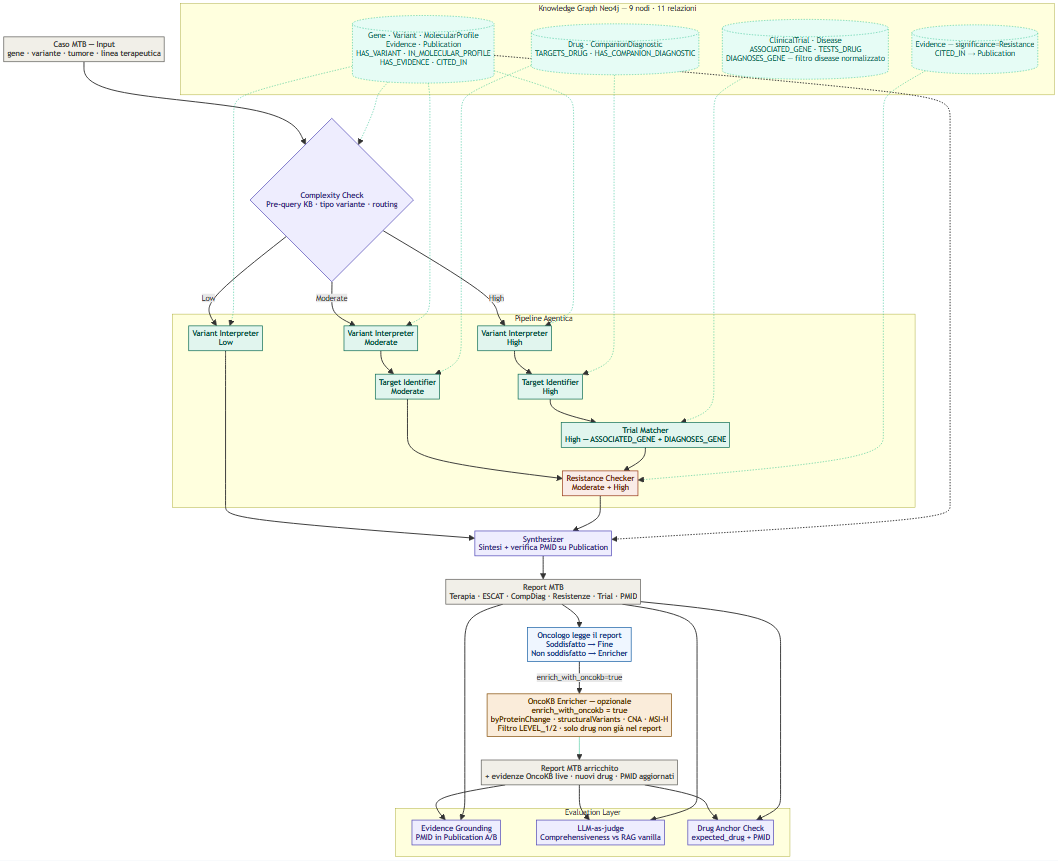
\includegraphics[width=0.98\textwidth]{pipeline_mtb_v3.png}
\caption{Diagramma architetturale della pipeline agentica GraphRAG v3.1}
\label{fig:pipelinev3}
\end{figure}

La v3 introduce tre aggiornamenti: (i) l'\textbf{OncoKB Enricher}, nodo opzionale post-report attivato con \code{enrich\_with\_oncokb=true} secondo un pattern \emph{human-in-the-loop}; (ii) l'integrazione di DIAGNOSES\_GENE nel Trial Matcher (il conteggio delle relazioni mappate sale a 11); (iii) un Complexity Check migliorato che considera \code{alteration\_type}. Lo schema di input clinico \`e stato formalizzato.

\begin{center}
\small
\begin{tabularx}{\textwidth}{@{}>{\ttfamily}l l X c@{}}
\toprule
\normalfont\bfseries Campo & \bfseries Tipo & \bfseries Valori ammessi & \bfseries Obbl. \\
\midrule
gene & string & HUGO symbol (null per biomarker agnostici) & S\`i* \\
variant & string & Protein change, Fusion, MSI-High, TMB-High & S\`i \\
tumor\_type & string & Nome tumore o codice OncoTree & S\`i \\
alteration\_type & enum & point\_mutation\,|\,fusion\,|\,cna\,|\,itd\,|\,atypical\,|\,biomarker & S\`i \\
therapy\_line & string & first / second / later-line & No \\
enrich\_with\_oncokb & bool & true / false (default false) & No \\
\bottomrule
\end{tabularx}
\end{center}
\noindent {\footnotesize *Il campo \code{category} del benchmark \`e escluso dall'input a runtime: \`e un metadato di classificazione e inserirlo provocherebbe overfitting nella valutazione. Il \code{Complexity Check} resta affidato a un LLM flessibile per preservare la generalizzabilit\`a.}

\subsection{Verifica delle query Cypher per \code{alteration\_type}}
Oltre 15 query Neo4j hanno verificato la fattibilit\`a del Variant Interpreter su tutti e sei i tipi di alterazione. Le point mutation seguono il percorso classico Gene\,$\to$\,Variant\,$\to$\,MP\,$\to$\,Evidence; gli altri tipi richiedono ricerca diretta su \code{MolecularProfile.name} via \code{CONTAINS}.

\begin{center}
\small
\begin{tabularx}{\textwidth}{@{}>{\ttfamily\bfseries\color{primary}}l c X@{}}
\toprule
\normalfont\bfseries\color{primary} Tipo & \bfseries Casi & \bfseries Percorso di query / nota \\
\midrule
point\_mutation & 14 & Gene\,$\to$\,Variant\,$\to$\,MP\,$\to$\,Evidence (percorso classico) \\
fusion & 6 & \code{MolecularProfile.name CONTAINS gene} (es. \code{v::ALK Fusion}) \\
atypical & 4 & \code{MolecularProfile.name CONTAINS 'Exon X'} \\
cna & 3 & nome contiene gene + ``amplif''/``deletion''; \bench{030} \`e un GAP \\
itd & 1 & \bench{010} FLT3 ITD: 23 evidenze totali su AML e APL \\
biomarker & 2 & ``TMB High'' / ``MSI High'' (richiedono mapping verso le API) \\
\bottomrule
\end{tabularx}
\end{center}

\begin{insightbox}[Tre implicazioni per l'implementazione]
\begin{enumerate}[leftmargin=1.4em]
\item \textbf{Branching obbligatorio} per \code{alteration\_type}: non esiste una query Cypher unica; in LangGraph sar\`a un conditional edge o un if/else interno.
\item \textbf{Priorit\`a ai profili semplici} rispetto ai composti (es. \code{BCR::ABL1 Fusion AND ABL1 T315I}): match esatto privilegiato, ordinando con \code{ORDER BY size(mp.name) ASC}.
\item \textbf{Dizionario di mapping KB\,$\leftrightarrow$\,OncoKB}: il database locale usa ``TMB High''/``MSI High'', le API ``TMB-H''/``MSI-H''; serve un dizionario di conversione esplicito.
\end{enumerate}
\end{insightbox}

% ========================================================
% PART V
% ========================================================
\part{Valutazione e risultati sperimentali}

\section{Metodologia di valutazione}

\subsection{Cosa stiamo davvero misurando}
Durante lo sviluppo \`e emerso un dubbio fondamentale: il benchmark con la sola colonna \code{expected\_drug} misura se il sistema ``ha individuato il farmaco corretto'', ma questo non \`e l'obiettivo reale. Un oncologo del MTB non ha bisogno che gli si suggerisca ``somministra Osimertinib'': conosce gi\`a la scelta standard. Il valore aggiunto \`e nella \emph{giustificazione strutturata, completa e referenziata}.

\begin{center}
\small
\begin{tabularx}{\textwidth}{@{}p{4.6cm} X@{}}
\toprule
\bfseries\color{gapred} Output povero & \bfseries\color{passgreen} Output utile \\
\midrule
``Raccomandazione: Osimertinib'' (mero esercizio di classificazione) &
``Osimertinib, evidenza A in CIViC per EGFR L858R in NSCLC; evidenze B per Erlotinib e Gefitinib; resistenza acquisita T790M (su cui Osimertinib resta attivo); 3 trial aperti, uno in fase III; evidenza primaria FLAURA, PMID 29151359.'' \\
\bottomrule
\end{tabularx}
\end{center}

\subsection{Valutazione a due livelli}
Si mantiene il benchmark dei 30 casi come ancora quantitativa (\emph{Drug Anchor}: Top-1/Top-3 accuracy) e vi si affianca una rubrica qualitativa semi-automatica applicata con LLM-as-judge. Il confronto isola il contributo del KG mettendo a paragone tre configurazioni: (A) LLM zero-shot, (B) RAG vanilla su testo, (C) GraphRAG agentico.

\subsection{La rubrica LLM-as-judge ricalibrata}
La rubrica iniziale a 5 criteri conteneva un criterio ``struttura'' che restituiva sistematicamente 5.0 (il Synthesizer impone una formattazione fissa), gonfiando in modo fittizio la media. \`E stata rimossa e i criteri ridefiniti a 4, ancorati alla letteratura.

\begin{center}
\small
\begin{tabularx}{\textwidth}{@{}>{\bfseries\color{primary}}l p{3.1cm} X@{}}
\toprule
Criterio & Ispirazione & Descrizione \\
\midrule
Completezza & Edge et al., 2025 & Copre variante, terapia, resistenze e trial? \\
Utilit\`a clinica & Edge et al., 2025 & Immediata usabilit\`a al board (assorbe leggibilit\`a/struttura) \\
Fedelt\`a evidenze & Wu et al., 2024 & I PMID citati sono nel KG e pertinenti? \\
Accuratezza clinica & Criterio originale & Precisione di farmaci, CDx e tiering ESCAT \\
\bottomrule
\end{tabularx}
\end{center}

\subsection{La gerarchia delle metriche}
Le metriche sono organizzate per importanza e originalit\`a: (1) \textbf{Evidence Grounding} [metrica originale]; (2) \textbf{LLM-as-judge} su Comprehensiveness/Diversity/Actionability [ispirato a Edge]; (3) \textbf{Drug Anchor + Primary Citation} [sanity check]; (4) \textbf{metriche Trial Matcher} (NDCG@10, P@10, AUROC) [ispirato a Jin].

\section{Risultati sperimentali}

\subsection{Confronto Caso per Caso: I 30 Benchmark}
La Tabella \ref{tab:comparison_cases} riporta l'esecuzione integrale della pipeline valutativa sui 30 casi clinici estratti da OncoKB.

\begin{table}[htbp]
\centering
\footnotesize
\setlength{\tabcolsep}{4pt}
\renewcommand{\arraystretch}{1.1}
\caption{Confronto Caso per Caso: GraphRAG vs Zero-Shot (Giudice: MiniMax-M2.5)}
\label{tab:comparison_cases}
\begin{tabularx}{\textwidth}{l >{\raggedright\arraybackslash}X >{\raggedright\arraybackslash}X l c c r}
\toprule
\rowcolor{primaryblue}
\color{white}\textbf{ID} & \color{white}\textbf{Gene/Variante} & \color{white}\textbf{Tumore} & \color{white}\textbf{Categoria} & \color{white}\textbf{GR} & \color{white}\textbf{ZS} & \color{white}\textbf{$\Delta$ (GR-ZS)} \\
\midrule
\bench{BENCH-001} & EGFR L858R & NSCLC & baseline & 4.00 & 4.25 & \fail{-0.25} \\
\rowcolor{roweven} \bench{BENCH-002} & ALK Fusion & NSCLC & baseline & 4.12 & 4.40 & \fail{-0.28} \\
\bench{BENCH-003} & BRAF V600E & Melanoma & baseline & 4.25 & 3.12 & \pass{+1.12} \\
\rowcolor{roweven} \bench{BENCH-004} & ERBB2 Amplification & Breast Cancer HER2+ & baseline & 4.38 & 4.12 & \pass{+0.26} \\
\bench{BENCH-005} & BRCA1 Mutation & Ovarian Cancer & baseline & 3.12 & 4.12 & \fail{-1.00} \\
\rowcolor{roweven} \bench{BENCH-006} & ABL1 BCR-ABL1 Fusion & CML & baseline & 3.38 & 3.88 & \fail{-0.50} \\
\bench{BENCH-007} & BRAF V600E & Colorectal Cancer & baseline & 3.75 & 3.88 & -0.12 \\
\rowcolor{roweven} \bench{BENCH-008} & PIK3CA Mutation & Breast Cancer HR+ & baseline & 4.25 & 4.25 & +0.00 \\
\bench{BENCH-009} & KIT Exon 11 Mutation & GIST & baseline & 2.88 & 3.25 & \fail{-0.38} \\
\rowcolor{roweven} \bench{BENCH-010} & FLT3 ITD & AML & baseline & 3.25 & 3.88 & \fail{-0.62} \\
\bench{BENCH-011} & EGFR T790M & NSCLC & resistance & 3.88 & 4.12 & \fail{-0.25} \\
\rowcolor{roweven} \bench{BENCH-012} & KRAS G12C & NSCLC & new\_target & 3.25 & 4.38 & \fail{-1.12} \\
\bench{BENCH-013} & ALK G1202R & NSCLC & resistance & 1.62 & 3.40 & \fail{-1.77} \\
\rowcolor{roweven} \bench{BENCH-014} & ABL1 T315I & CML & resistance & 4.50 & 4.62 & -0.12 \\
\bench{BENCH-015} & RET Fusion & NSCLC & new\_target & 4.25 & 3.50 & \pass{+0.75} \\
\rowcolor{roweven} \bench{BENCH-016} & NTRK1 Fusion & Solid Tumor & tumor\_agnostic & 4.38 & 4.50 & -0.12 \\
\bench{BENCH-017} & MMR MSI-High & Colorectal Cancer & biomarker & 3.25 & 4.62 & \fail{-1.38} \\
\rowcolor{roweven} \bench{BENCH-018} & KRAS G12C & Colorectal Cancer & new\_target & 3.25 & 4.50 & \fail{-1.25} \\
\bench{BENCH-019} & KIT Exon 9 Mutation & GIST & resistance & 4.38 & 3.50 & \pass{+0.88} \\
\rowcolor{roweven} \bench{BENCH-020} & BRAF V600E & NSCLC & off\_label & 3.25 & 3.75 & \fail{-0.50} \\
\bench{BENCH-021} & ERBB2 Amplification & Gastric Cancer & off\_label & 3.88 & 3.38 & \pass{+0.50} \\
\rowcolor{roweven} \bench{BENCH-022} & BRCA2 Mutation & Prostate Cancer & off\_label & 3.50 & 3.75 & \fail{-0.25} \\
\bench{BENCH-023} & TMB TMB-High & Solid Tumor & tumor\_agnostic & 3.88 & 3.75 & +0.12 \\
\rowcolor{roweven} \bench{BENCH-024} & EGFR Exon 19 Deletion & NSCLC & baseline & 3.62 & 3.38 & \pass{+0.25} \\
\bench{BENCH-025} & IDH1 R132 & AML & new\_target & 1.62 & 3.88 & \fail{-2.25} \\
\rowcolor{roweven} \bench{BENCH-026} & FGFR2 Fusion & Cholangiocarcinoma & new\_target & 4.25 & 3.62 & \pass{+0.62} \\
\bench{BENCH-027} & MET Exon 14 Skipping & NSCLC & new\_target & 3.38 & 3.00 & \pass{+0.38} \\
\rowcolor{roweven} \bench{BENCH-028} & ROS1 Fusion & NSCLC & new\_target & 4.12 & 4.00 & +0.12 \\
\bench{BENCH-029} & BRAF V600E & Thyroid Cancer & off\_label & 4.00 & 4.25 & \fail{-0.25} \\
\rowcolor{roweven} \bench{BENCH-030} & ERBB2 Amplification & Gastric Cancer & new\_target & 4.62 & 4.50 & +0.12 \\
\bottomrule
\end{tabularx}
\end{table}

\subsection{Benchmark ricalcolato (v2)}
Sui 30 casi, lo score medio resta \textbf{3.96/5.0} (stabile rispetto alla v1): la rimozione del bias ``struttura'' ha allineato la valutazione a criteri pi\`u severi, e la stabilit\`a dimostra la robustezza del sistema. La scomposizione per criterio:

\begin{center}
\begin{tikzpicture}
\begin{axis}[
  width=12.5cm, height=5.2cm,
  xbar, xmin=0, xmax=5,
  bar width=13pt,
  enlarge y limits=0.28,
  symbolic y coords={Utilit\`a clinica,Accuratezza clinica,Completezza,Fedelt\`a evidenze},
  ytick=data,
  nodes near coords, nodes near coords align={horizontal},
  every node near coord/.append style={font=\footnotesize\sffamily,color=inkgray},
  xlabel={\footnotesize\sffamily score medio (1--5)},
  tick label style={font=\footnotesize\sffamily},
  axis line style={rulec}, grid=major, grid style={rulec!50},
]
\addplot[fill=secondary,draw=secondary] coordinates {
  (3.59,Utilit\`a clinica) (3.80,Accuratezza clinica) (4.00,Completezza) (4.48,Fedelt\`a evidenze)};
\end{axis}
\end{tikzpicture}
\end{center}

\begin{tesibox}[Key finding per RQ2]
Il divario tra la fedelt\`a delle fonti (4.48) e l'utilit\`a clinica pratica (3.59) mostra che, sebbene la base dati strutturata garantisca il rigore bibliografico, la \emph{traduzione automatica} delle evidenze grezze in indicazioni operative \`e lo snodo critico dell'ingegneria dei sistemi GraphRAG in ambito medico.
\end{tesibox}

\subsection{OncoKB Enricher sui casi critici}
I tre casi con score inferiore a 3.0 sono stati rieseguiti abilitando l'arricchimento live.

\begin{center}
\small
\begin{tabular}{@{}llccc l@{}}
\toprule
Caso & Profilo & Base & Arricch. & $\Delta$ & Esito \\
\midrule
\bench{013} & ALK G1202R / NSCLC & 1.25 & \textbf{4.60} & \color{passgreen}+3.35 & GAP risolto \\
\bench{018} & KRAS G12C / CRC & 2.75 & \textbf{4.25} & \color{passgreen}+1.50 & Errore corretto \\
\bench{027} & MET Exon 14 / NSCLC & 2.88 & 2.88 & +0.00 & Limite arch. \\
\bottomrule
\end{tabular}
\end{center}

\noindent \bench{018} \`e particolarmente istruttivo: il sistema base raccomandava Cetuximab in monoterapia per un CRC KRAS G12C, clinicamente \emph{controindicato} (KRAS \`e biomarcatore di resistenza agli anti-EGFR). L'Enricher ha fornito le evidenze \code{LEVEL\_1} per Sotorasib e Adagrasib. Il caso \bench{027} mostra il limite dell'arricchimento \emph{additivo}: non corregge errori citazionali preesistenti nel database locale.

\subsection{RQ1: GraphRAG vs Zero-shot e il bias del giudice}
La prima run usava Gemma come giudice --- lo stesso modello dello zero-shot vanilla --- producendo un vistoso bias di auto-valutazione (delta apparente $-0.722$ a favore dello zero-shot). Ripetendo con un giudice indipendente (MiniMax M2.5) il gap si riduce di $2.7\times$ (delta reale $-0.264$). \`E un'evidenza empirica di rilievo sui limiti dell'LLM-as-judge, che \`e stato di conseguenza retrocesso a metrica secondaria a favore delle metriche oggettive.

\subsection{Allucinazione bibliografica dello zero-shot}
Tutti i PMID citati nei 30 report zero-shot sono stati verificati contro PubMed/NCBI E-utilities.

\begin{warnbox}[Il risultato chiave di RQ1]
\textbf{Tasso di allucinazione clinica bibliografica: 100\%} (115/115 PMID). Il 96.52\% dei codici esiste su PubMed ma tratta argomenti del tutto scorrelati (dall'istruzione superiore alle emulsioni stabilizzate); solo il 3.48\% \`e del tutto inventato. I PMID dello zero-shot sono ``token decorativi'' privi di valore referenziale.
\end{warnbox}

\noindent A titolo di esempio citabile in tesi: per \bench{001} (EGFR L858R / NSCLC) lo zero-shot cita il PMID 29703322, il cui titolo reale \`e ``\emph{Disruptive trends in higher education: Leadership skills for successful leaders}''.

\subsection{Retrieval Pollution e mitigazione}
Il \emph{retrieval pollution} si verifica quando le informazioni generali di gene (es. sensibilit\`a di EGFR L858R a Erlotinib) inquinano il contesto per varianti specifiche di resistenza (es. EGFR T790M). La v3.1 introduce nel \code{resistance\_checker.py} un filtro variante-specifico (\code{CYPHER\_EXCLUDE\_DRUGS}) che esclude preventivamente i farmaci inquinanti. Il Safety Pass Rate automatico sale da 86.7\% a 90.0\%; la safety clinica reale, al netto dei falsi negativi della regex, \`e del 96.7\%.

\begin{tesibox}
I due falsi negativi (\bench{013}, \bench{014}) menzionano i farmaci controindicati \emph{solo} nella descrizione del profilo di resistenza (contesto informativo) e non come raccomandazione attiva --- comportamento clinicamente corretto che il check string-matching non distingue.
\end{tesibox}

\subsection{Confronto a tre vie finale}
Il confronto oggettivo sull'intero benchmark sintetizza il profilo di rischio opposto dei due approcci.

\begin{center}
\begin{tikzpicture}
\begin{axis}[
  width=13cm, height=6cm,
  ybar, bar width=11pt,
  ymin=0, ymax=119,
  enlarge x limits=0.22,
  symbolic x coords={Therapeutic Match,Evidence Grounding,Safety Pass},
  xtick=data,
  nodes near coords, nodes near coords align={vertical},
  every node near coord/.append style={font=\scriptsize\sffamily,color=inkgray},
  ylabel={\footnotesize\sffamily valore (\%)},
  tick label style={font=\footnotesize\sffamily},
  legend style={at={(0.5,-0.25)},anchor=north,legend columns=3,font=\footnotesize\sffamily,draw=rulec},
  axis line style={rulec}, grid=major, grid style={rulec!50},
]
\addplot[fill=gapred!75,draw=gapred] coordinates {(Therapeutic Match,100) (Evidence Grounding,0) (Safety Pass,96.7)};
\addplot[fill=secondary,draw=secondary] coordinates {(Therapeutic Match,95) (Evidence Grounding,96.7) (Safety Pass,86.7)};
\addplot[fill=primary,draw=primary] coordinates {(Therapeutic Match,95) (Evidence Grounding,100) (Safety Pass,90)};
\legend{Zero-shot,GraphRAG base,GraphRAG + Enricher}
\end{axis}
\end{tikzpicture}
\end{center}

\begin{insightbox}[I tre finding scientifici cruciali]
\begin{enumerate}[leftmargin=1.4em]
\item \textbf{Verificabilit\`a (0\% vs 100\%):} lo zero-shot fornisce risposte corrette per memoria parametrica ma allucina i PMID; solo GraphRAG + Enricher garantisce tracciabilit\`a totale.
\item \textbf{Retrieval pollution (safety 86.7\% vs 96.7\%):} il recupero a livello di gene immette farmaci storici non pi\`u indicati per varianti di resistenza; lo zero-shot, privo di questo rumore, non compie l'errore. Un finding non banale.
\item \textbf{Bias del benchmark:} il Therapeutic Match perfetto dello zero-shot (1.000) rivela che i casi sono ad alta ricorrenza in letteratura, facilitando la memoria parametrica.
\end{enumerate}
\end{insightbox}

\noindent Metriche oggettive definitive (post-fix ESCAT): \textbf{Drug Anchor Check} 96.7\% (29/30) per entrambi i sistemi; \textbf{PMID Coverage Rate} 60.0\% per GraphRAG (0\% zero-shot); \textbf{ESCAT Tier Match} 100.0\% (vs 0\%); \textbf{PMID Hallucination Rate} 0.0\% per GraphRAG (vs 100.0\% dello zero-shot).

\subsection{Ottimizzazione strutturale dell'ESCAT Interpreter}
La prima iterazione dell'ESCAT Interpreter usava una mappatura statica dei livelli di evidenza (\code{A $\to$ I-A, B $\to$ II-B}) che produceva errori sistematici, fermando lo score al 73.3\%. Il problema di fondo era l'assenza di confronto tra l'istologia dell'evidenza e quella del paziente (condizione necessaria secondo le linee guida ESMO). 
Per questo \`e stato implementato un \emph{fix} a tre livelli:
\begin{enumerate}
\item \textbf{Fuzzy Matching Istologico:} introduzione della funzione \code{\_is\_same\_tumor()} per verificare le inclusioni semantiche tra il campo \code{disease} del grafo e l'input del paziente.
\item \textbf{Fallback Contestuale:} abbandono della mappa statica. Se l'istologia differisce, l'evidenza viene degradata automaticamente per via del contesto \emph{off-label} (da \code{A/B} a \code{II-B}); se l'evidenza ha \code{significance = Resistance}, viene declassata e mai associata a Tier predittivi di efficacia.
\item \textbf{Prompt Iniection:} inserimento del flag booleano \code{Match istologico: SI/NO} per ciascuna evidenza direttamente nel prompt del generatore.
\end{enumerate}
Questi interventi correttivi hanno eliminato gli errori per le varianti tumor-agnostic e di resistenza, portando la \emph{Tier Match accuracy} al \textbf{100.0\%} sui 30 casi del benchmark.

\subsection{Analisi Casi Drug Anchor Check --- Finding Narrativo Chiave}
Sebbene il Drug Anchor Check sia identico per entrambi i sistemi (96.7\%, 29/30 casi), gli errori sono \textbf{diversi e asimmetrici}, illustrando il rischio clinico dell'approccio zero-shot:
\begin{itemize}
\item \textbf{BENCH-004 (GraphRAG sbaglia, Zero-Shot indovina):} ERBB2 Amplificazione nel tumore al seno. GraphRAG non restituisce la combinazione attesa (Trastuzumab + Pertuzumab) per un errore tecnico: mancava il nodo della combinazione nella KB (identificato come bug e risolto). Lo Zero-Shot indovina grazie alla memoria parametrica su un protocollo storico consolidato.
\item \textbf{BENCH-018 (Zero-Shot sbaglia, GraphRAG indovina):} KRAS G12C nel tumore del Colon-Retto. Questo caso illustra esattamente il rischio clinico del LLM \emph{vanilla} in oncologia di precisione. Lo Zero-Shot raccomanda Sotorasib in monoterapia, che \`e lo standard per il carcinoma polmonare (NSCLC), ignorando totalmente che nel colon-retto l'inibizione di KRAS G12C causa una riattivazione del feedback mediato da EGFR. Questo rende obbligatorio associare un anti-EGFR (es.\ Panitumumab), approvazione FDA agosto 2023 basata sul trial CodeBreaK 300 (NEJM 2023). Un medico che usasse lo zero-shot riceverebbe una raccomandazione clinicamente pericolosa. GraphRAG, basandosi sulle relazioni strutturate del Knowledge Graph che codificano la specificit\`a istologica, fornisce la raccomandazione corretta, dimostrandosi immune al bias statistico dei dati di training.
\end{itemize}
Il caso \bench{018} mostra il limite clinico dello zero-shot: il bias da distribuzione dei dati di training sovrascrive le specificit\`a istologiche, portando a raccomandazioni potenzialmente pericolose.

\subsection{Lettura Corretta dei Risultati (LLM-as-judge)}
I risultati qualitativi con LLM-as-judge sembrano premiare lo zero-shot (Score totale 3.92 vs 3.72 di GraphRAG), ma questo rivela un vistoso \emph{fluency bias}. Lo zero-shot ottiene 4.13 in ``Fedelt\`a alle Evidenze'' pur avendo un tasso di allucinazione dei PMID del 100\%: il giudice LLM valuta la fluidit\`a percepita del testo, non la correttezza fattuale delle fonti. Sulle metriche oggettive e verificabili, GraphRAG domina nettamente.

% ========================================================
% ETHICS & CONCLUSIONS
% ========================================================
\section{Considerazioni etiche e limiti}
\begin{itemize}
\item Il sistema \`e un \emph{decision support}, non un decision maker: le raccomandazioni vanno discusse in sede di MTB con giudizio clinico umano.
\item Non \`e un dispositivo medico ai sensi della normativa MDR/IVDR; non si pone l'obiettivo della certificazione regolatoria in fase di tesi.
\item OncoKB: i termini di servizio vietano l'uso dei dati per il training di modelli; il progetto usa il dump statico per il KG offline e chiamate API live solo a runtime su attivazione esplicita.
\item I database curati sono \emph{lagging indicators}: di qui l'integrazione live (ClinicalTrials.gov, OncoKB).
\item Bias di rappresentazione (genomica dominata da popolazioni occidentali) e long-tail variants con evidenze deboli: il sistema deve segnalarlo esplicitamente.
\item L'uso su dati di pazienti reali richiederebbe approvazione del Comitato Etico e gestione GDPR.
\end{itemize}

\section{Conclusioni e lavori futuri}
La narrazione del progetto si colloca all'intersezione tra tre tendenze convergenti: la validazione clinica dell'uso di ESCAT come standard MTB (Aldea et al., IASLC 2025), la dimostrazione che il RAG testuale soffra di limitazioni strutturali nella gestione delle citazioni (Berman et al., JMIR 2025), e la validazione industriale su larga scala che la KB oncologica strutturata + agenti LLM specializzati riduca enormemente le allucinazioni rispetto al solo LLM (Loaiza-Bonilla et al., ESMO 2026). Questa tesi contribuisce con una pipeline open-source completa che integra la classificazione ESCAT contestuale e la verifica strutturale delle citazioni --- elementi assenti o solo parziali in tutti e tre i sistemi di riferimento.

Il lavoro ha portato il progetto dalla sola infrastruttura a un sistema agentico valutato. La narrativa della tesi si struttura attorno a quattro \emph{finding} originali.

\begin{defbox}[I quattro pilastri della tesi]
\begin{enumerate}[leftmargin=1.4em]
\item \textbf{Allucinazione bibliografica sistematica (100\%)} dello zero-shot: la verificabilit\`a delle fonti \`e l'unico requisito non negoziabile in clinica.
\item \textbf{Retrieval pollution clinico:} i sistemi RAG, se interpellati a livello di gene, inquinano il contesto con farmaci non efficaci per varianti resistenti.
\item \textbf{Enricher live come knowledge fall-back:} l'integrazione ibrida risolve i gap strutturali locali garantendo il grounding.
\item \textbf{Safety automatica vs safety reale:} dimostrazione quantitativa del limite delle metriche string-matching nella valutazione della sicurezza clinica.
\end{enumerate}
\end{defbox}

\noindent \textbf{Prossimi passi.} (i) Misurare il tasso di allucinazione bibliografica dello zero-shot anche via verifica PubMed sistematica; (ii) raffinare il Resistance Checker con regole di filtraggio rigido per scartare i farmaci storici controindicati; (iii) sviluppare un classificatore semantico per il Safety Check che isoli le menzioni informative dai falsi negativi delle regex; (iv) consolidare il ``Clinical Correctness Score'' ($\mathrm{TM}\times\mathrm{EG}\times\mathrm{Safety}$) come metrica oggettiva primaria; (v) redigere la sezione metodologica della tesi descrivendo i 4 criteri e la base scientifica associata.

\vspace{8pt}
\begin{center}
{\color{rulec}\rule{0.5\textwidth}{0.6pt}}\\[4pt]
{\sffamily\footnotesize\color{inkgray} Fine del report --- sintesi del lavoro dal 29 maggio all'8 giugno 2026}
\end{center}

% ========================================================
% GLOSSARY
% ========================================================
\section{Glossario e acronimi}
\addcontentsline{toc}{section}{Glossario e acronimi}
\markboth{Glossario e acronimi}{}
Di seguito si riporta il glossario completo dei termini scientifici, degli acronimi medici, dei geni bersaglio e delle sigle oncologiche utilizzate nel report e nelle valutazioni del benchmark.

\begin{description}[leftmargin=1.4em,style=nextline]
\item[ABL1] \emph{ABL Proto-Oncogene 1, Non-Receptor Tyrosine Kinase}. Gene coinvolto nella fusione \code{BCR::ABL1}, target primario dell'imatinib nella leucemia mieloide cronica.
\item[ALK] \emph{ALK Receptor Tyrosine Kinase} (Chinasi del Linfoma Anaplastico). Oncogene coinvolto in fusioni patogenetiche e varianti di resistenza secondarie (es.\ G1202R) nel tumore al polmone.
\item[AML] \emph{Acute Myeloid Leukemia} (Leucemia Mieloide Acuta). Neoplasia del sistema emopoietico ad alta aggressività, analizzata nel benchmark su target quali \code{FLT3} (ITD) e \code{IDH1} (R132).
\item[AMP/ASCO/CAP] Linee guida congiunte delle principali società di patologia molecolare e oncologia americane (\emph{Association for Molecular Pathology, American Society of Clinical Oncology, College of American Pathologists}) per la classificazione clinica delle alterazioni genomiche nei tumori solidi.
\item[API] \emph{Application Programming Interface} (Interfaccia di Programmazione delle Applicazioni). Canale di connessione software usato a runtime per interrogare live i registri OncoKB e ClinicalTrials.gov.
\item[atypical] Classe di alterazione utilizzata nel benchmark (\code{alteration\_type}) per identificare varianti molecolari complesse che non corrispondono a singole mutazioni puntiformi ma coinvolgono interi esoni o domini (es.\ mutazioni degli esoni 9 o 11 di \code{KIT}, skipping dell'esone 14 di \code{MET}).
\item[biomarker] Classe di alterazione utilizzata nel benchmark (\code{alteration\_type}) per identificare marcatori biologici o quantitativi indipendenti da un singolo gene specifico, che descrivono invece profili genomici complessi o sistemici (es.\ \code{TMB-High} o \code{MSI-High}).
\item[BRAF] \emph{B-Raf Proto-Oncogene, Serine/Threonine Kinase}. Oncogene della via MAPK; la mutazione \code{V600E} è un target d'elezione nel melanoma e nel colon-retto.
\item[BRCA1 / BRCA2] Geni oncosoppressori (\emph{Breast Cancer gene 1/2}) responsabili del meccanismo di riparazione del DNA per ricombinazione omologa; bersagli ideali degli inibitori di PARP (es.\ Olaparib).
\item[CDx] \emph{Companion Diagnostic} (Diagnostica d'accompagnamento). Test in vitro approvato congiuntamente ad un farmaco specifico al fine di identificare i pazienti idonei alla terapia.
\item[CGI] \emph{Conoscenza Gap Index}. Metrica normalizzata formulata in tesi per misurare la discrepanza informativa tra le interazioni molecolari di DGIdb e le evidenze cliniche di CIViC.
\item[CIViC] \emph{Clinical Interpretation of Variants in Cancer}. Database pubblico, collaborativo e curato da esperti per l'interpretazione clinica delle varianti somatiche nel cancro.
\item[CML] \emph{Chronic Myeloid Leukemia} (Leucemia Mieloide Cronica). Disordine mieloproliferativo caratterizzato dal cromosoma Philadelphia (\code{BCR::ABL1}), trattato con inibitori di tirosin-chinasi.
\item[CNA] \emph{Copy Number Alteration} (Alterazione del Numero di Copie). Aberrazione genomica che determina l'amplificazione o la delezione di porzioni cromosomiche. Rappresenta anche una classe di alterazione nel benchmark (\code{alteration\_type}), come l'amplificazione di \code{ERBB2}.
\item[CRC] \emph{Colorectal Cancer} (Carcinoma del Colon-Retto). Neoplasia intestinale analizzata nel benchmark in relazione a mutazioni di \code{KRAS} (G12C), \code{BRAF} (V600E) e instabilità microsatellitare.
\item[CYPHER] Linguaggio dichiarativo di interrogazione proprietario del database a grafo Neo4j, usato in tesi per navigare le relazioni molecolari del Knowledge Graph.
\item[DGIdb] \emph{Drug-Gene Interaction Database}. Risorsa pubblica ad accesso aperto che raccoglie e normalizza le interazioni note tra farmaci e geni da letteratura e database.
\item[DOID] \emph{Disease Ontology Identifier}. Identificativo controllato e univoco per l'ontologia delle malattie umane, usato per la normalizzazione dei nodi \code{Disease}.
\item[EGFR] \emph{Epidermal Growth Factor Receptor} (Recettore del Fattore di Crescita Epidermico). Recettore tirosin-chinasico sovraespresso o mutato nel tumore del polmone non a piccole cellule.
\item[ERBB2] \emph{Erb-B2 Receptor Tyrosine Kinase 2} (noto anche come HER2). Target amplificato in tumori mammari e gastrici, bersaglio di anticorpi monoclonali (Trastuzumab, Pertuzumab).
\item[ESCAT] \emph{ESMO Scale for Clinical Actionability of molecular Targets}. Scala standardizzata di classificazione dell'azionabilità clinica dei target genomici in base alle evidenze scientifiche.
\item[ESMO] \emph{European Society for Medical Oncology} (Società Europea di Oncologia Medica). Associazione professionale di riferimento per lo sviluppo di linee guida cliniche in Europa.
\item[ETL] \emph{Extract, Transform, Load} (Estrazione, Trasformazione, Caricamento). Pipeline software per l'ingestion ed il consolidamento dei database biologici all'interno di Neo4j.
\item[FDA] \emph{Food and Drug Administration}. Agenzia governativa statunitense per la regolamentazione di prodotti alimentari, farmaceutici e dispositivi medici diagnostici.
\item[FGFR2] \emph{Fibroblast Growth Factor Receptor 2}. Recettore tirosin-chinasico; le sue fusioni rappresentano un target terapeutico recente nel colangiocarcinoma.
\item[FLT3] \emph{Fms Related Receptor Tyrosine Kinase 3}. Recettore tirosin-chinasico espresso in cellule emopoietiche progenitorie; mutazioni come l'ITD guidano la terapia mirata in AML.
\item[fusion] Classe di alterazione utilizzata nel benchmark (\code{alteration\_type}) per identificare fusioni geniche derivanti da riarrangiamenti strutturali cromosomici che uniscono porzioni di due geni distinti (es.\ fusioni di \code{ALK}, \code{ROS1}, \code{RET} o \code{NTRK1}).
\item[GDPR] \emph{General Data Protection Regulation}. Regolamento generale europeo sulla protezione dei dati, stringente vincolo etico per l'eventuale implementazione clinica con dati reali dei pazienti.
\item[GIST] \emph{Gastrointestinal Stromal Tumor} (Tumore Stromale Gastrointestinale). Neoplasia mesenchimale del tratto gastrointestinale legata a mutazioni attivanti dei geni \code{KIT} o \code{PDGFRA}.
\item[GraphRAG] Evoluzione del paradigma RAG che utilizza database a grafo per contestualizzare la generazione di testo da parte di modelli LLM attraverso percorsi semantici strutturati.
\item[HHI] \emph{Herfindahl-Hirschman Index}. Indice di concentrazione economica, riadattato in tesi per valutare quantitativamente il curation bias (squilibrio editoriale) sui geni della KB.
\item[HRD] \emph{Homologous Recombination Deficiency} (Deficienza della Ricombinazione Omologa). Biomarcatore molecolare indicante il deficit di riparazione del DNA per ricombinazione omologa, bersaglio clinico degli inibitori di PARP.
\item[IDH1] \emph{Isocitrate Dehydrogenase 1} (Isocitrato Deidrogenasi 1). Enzima mutato nel citoplasma di cellule leucemiche in AML (variante \code{R132}), bersaglio dell'ivosidenib.
\item[ITD] \emph{Internal Tandem Duplication} (Duplicazione Interna in Tandem). Aberrazione strutturale con duplicazione ripetuta in sequenza, tipica e prognostica del gene \code{FLT3} in AML. Rappresenta anche una classe di alterazione nel benchmark (\code{alteration\_type}), es.\ \code{FLT3-ITD}.
\item[KG] \emph{Knowledge Graph} (Grafo della Conoscenza). Rete di entità collegate da relazioni tipizzate, impiegata per memorizzare la conoscenza clinica oncologica in Neo4j.
\item[KIT] \emph{KIT Proto-Oncogene, Receptor Tyrosine Kinase}. Recettore tirosin-chinasico associato all'oncogenesi dei GIST (es.\ mutazioni dell'esone 9 o 11).
\item[KRAS] \emph{KRAS Proto-Oncogene, GTPase}. Oncogene centrale della via RAS/MAPK, storicamente ritenuto non targettabile e recentemente aggredito (es.\ mutazione \code{G12C} in NSCLC e CRC).
\item[LLM] \emph{Large Language Model}. Modelli linguistici artificiali addestrati su enormi dataset testuali per comprendere, sintetizzare e generare linguaggio naturale o semi-strutturato.
\item[MDR/IVDR] Regolamenti dell'Unione Europea per i dispositivi medici (\emph{Medical Device Regulation}) e diagnostici in vitro (\emph{In Vitro Diagnostic Regulation}) per la marcatura CE dei sistemi software di supporto clinico.
\item[MET] \emph{MET Proto-Oncogene, Receptor Tyrosine Kinase}. Recettore tirosin-chinasico; alterazioni di skipping dell'esone 14 guidano terapie con inibitori specifici (es.\ Capmatinib).
\item[MMR] \emph{Mismatch Repair} (Riparazione del Disallineamento). Meccanismo cellulare di correzione degli errori di replicazione del DNA; la sua deficienza porta allo stato MSI-High.
\item[MSI-High / MSI-H] \emph{Microsatellite Instability High} (Instabilità Microsatellitare Elevata). Biomarcatore tumor-agnostic indicativo di elevata immunogenicità, bersaglio dell'immunoterapia (Pembrolizumab).
\item[MTB] \emph{Molecular Tumor Board}. Comitato oncologico multidisciplinare incaricato di analizzare i profili genomici complessi dei pazienti per formulare raccomandazioni terapeutiche personalizzate.
\item[NCT ID] \emph{National Clinical Trial Identifier}. Identificativo alfanumerico univoco (es.\ NCT00000000) assegnato a ciascun protocollo di sperimentazione clinica registrato su ClinicalTrials.gov.
\item[NGS] \emph{Next-Generation Sequencing} (Sequenziamento di Nuova Generazione). Tecnologia per il sequenziamento parallelo massivo degli acidi nucleici, sorgente primaria dei profili molecolari clinici.
\item[NSCLC] \emph{Non-Small-Cell Lung Cancer} (Carcinoma Polmonare Non a Piccole Cellule). La principale tipologia di tumore polmonare, fortemente caratterizzata da alterazioni molecolari targettabili (\code{EGFR}, \code{ALK}, \code{ROS1}, \code{RET}, \code{KRAS}).
\item[NTRK1 / NTRK2 / NTRK3] Geni recettoriali di neurotrofine. Le loro fusioni strutturali rappresentano uno dei primi biomarker interamente tumor-agnostic approvati FDA per terapie con larotrectinib.
\item[OncoKB] \emph{Oncology Knowledge Base}. Database MSKCC contenente informazioni cliniche curate per l'effetto biologico e l'azionabilità clinica di alterazioni tumorali somatiche.
\item[PIK3CA] \emph{Phosphatidylinositol-4,5-Bisphosphate 3-Kinase Catalytic Subunit Alpha}. Gene della subunità catalitica della chinasi PI3K, target primario nel carcinoma mammario HR+.
\item[PMID] \emph{PubMed Identifier}. Codice numerico univoco assegnato a ciascun articolo della letteratura biomedica indicizzato su MEDLINE/PubMed, utilizzato per calcolare l'Evidence Grounding.
\item[point\_mutation] Classe di alterazione utilizzata nel benchmark (\code{alteration\_type}) per indicare mutazioni puntiformi, ovvero variazioni di un singolo nucleotide che comportano la sostituzione di un singolo amminoacido nella proteina risultante (es.\ \code{EGFR L858R}, \code{BRAF V600E}).
\item[RAG] \emph{Retrieval-Augmented Generation}. Tecnica che unisce modelli linguistici generativi a sistemi di recupero informativo esterni per ridurre allucinazioni e incrementare la fattualità.
\item[RET] \emph{RET Proto-Oncogene}. Recettore tirosin-chinasico; le sue fusioni molecolari o mutazioni guidano terapie mirate con selpercatinib e pralsetinib.
\item[ROS1] \emph{ROS1 Proto-Oncogene, Receptor Tyrosine Kinase}. Oncogene chinasi; fusioni oncogeniche guidano sensibilità a inibitori TKI quali crizotinib ed entrectinib.
\item[TMB-High / TMB-H] \emph{Tumor Mutational Burden High} (Carico Mutazionale Elevato). Biomarcatore tumor-agnostic che quantifica le mutazioni somatiche per megabase di DNA sequenziato; indicatore di risposta all'immunoterapia.
\item[VHL] \emph{Von Hippel-Lindau Tumor Suppressor}. Gene oncosoppressore coinvolto nella degradazione di HIF-1. È il gene a massima densità di evidenza scientifica clinica nella KB.
\end{description}

% ========================================================
% REFERENCES
% ========================================================
\section*{Riferimenti bibliografici principali}
\addcontentsline{toc}{section}{Riferimenti bibliografici principali}
\small
\begin{description}[leftmargin=1.4em,style=nextline]
\item[Edge et al. (2025)] \emph{From Local to Global: A GraphRAG Approach to Query-Focused Summarization}. Microsoft Research, arXiv:2404.16130v2.
\item[Wu et al. (2024)] \emph{Medical Graph RAG: Towards Safe Medical Large Language Model via Graph Retrieval-Augmented Generation}. Oxford / CMU / Edinburgh, arXiv:2408.04187v2.
\item[Kim et al. (2024)] \emph{MDAgents: An Adaptive Collaboration of LLMs for Medical Decision-Making}. MIT / Google Research / Seoul National University, NeurIPS 2024.
\item[Jin et al. (2024)] \emph{Matching Patients to Clinical Trials with Large Language Models (TrialGPT)}. NIH/NCBI --- NCI --- University of Pittsburgh, Nature Communications 15:9074.
\item[Aldea et al. (2025)] \emph{IASLC Consensus Statement on Molecular Tumor Boards}. J Thorac Oncol. 2025;20:1594--1614.
\item[Berman et al. (2025)] \emph{RAG\_MTB: Retrieval-Augmented Generation for MTB}. JMIR Med Inform. 2025. PMID: 40053768.
\item[Loaiza-Bonilla et al. (2026)] \emph{OncoMultiAgentKB: A Neuro-Symbolic System}. ESMO Real World Data and Digital Oncology. 2026.
\end{description}

\end{document}